% Chapter 4: Application Studies
\chapter{Application Studies}
\label{chapter:skelcl-evaluation}

In this chapter we present various application studies evaluating the usefulness and performance of the abstractions introduced by the \SkelCL programming model which was presented in the previous section.
We start with a brief discussion of the experimental setup used throughout the chapter and discuss the metrics used to evaluate the \SkelCL programming model.
We will then look at applications from a wide range of application domains ranging from simple benchmark applications like the computation of the Mandelbrot set, over linear algebra and image processing applications, to real-world applications in medical imaging, physics, and biology.

For all application source codes using the \SkelCL library which are presented in this section we only show relevant sections and omit implementation details like initializing \SkelCL, including the correct set of header files, and prefix names with the \code{skelcl} namespace.

\section{Experimental Setup}
\label{sec:skelcl:experimental_setup}
This section briefly discusses the evaluation metrics used in this chapter which were chosen to measure the quality of the abstractions introduced in the \SkelCL programming model and their implementation in the \SkelCL library.
We will also discuss the hardware used in the experiments.


\subsection{Evaluation Metrics}
We want to evaluate the programmability, \ie, the ease of programming, and performance of the \SkelCL programming model and library.

Directly measuring programmability is difficult.
Various studies~\cite{HochsteinCSAB2005,HochsteinBVG2008} have been conducted and metrics~\cite{VanderwielNL1997} have been proposed to measure how convenient a certain style of programming or a certain programming model is.
None of these metrics is widely established in the scientific or industrial communities.
We chose to use one of the simples metrics possible to quantify programming effort: counting the \emph{Lines Of source Code} (LOC).
The author wants to emphasize that this metric is not always a good representation of programmability.
A shorter program does not necessarily mean that the development of the program has been more convenient.
We will, therefore, alongside presenting the lines of code argue \emph{why} the programming of parallel devices, like \GPUs, is easier as compared to the state-of-the-art approaches CUDA and OpenCL.
% These discussions will argue that code written using the \SkelCL programming approach has, besides ease of programming, other properties of high quality software including:
% high level of re-use, portability, 

As the metric for performance we use absolute and relative runtime.
%-- where possible --
We only make comparisons using software executed on the same hardware.
We perform comparisons using published software from researchers or officially provided by NVIDIA or AMD.
In addition, we use self developed and optimized CUDA and OpenCL code for comparisons versus the code written using the \SkelCL library.

\subsection{Hardware Setup}
For performing our runtime experiments we used a PC equipped with a quad-core \CPU (Intel Xeon E5520, 2.26\,GHz) and 12\,GB of main memory.
The system is connected to a Nvidia Tesla S1070 computing system consisting of four Nvidia Tesla \GPUs.
The S1070 has 16\,GB of dedicated memory (4\,GB per \GPU) which is accessed with up to 408\,GB/s (102\,GB/s per \GPU).
Each \GPU comprises 240 streaming processor cores running at up to 1.44\,GHz.
The Linux based Ubuntu operating system was used.
The runtime experiments where conducted at different times from 2010 until 2015.
For each experiment the latest Nvidia \GPU driver available was used.

This hardware setup represents a common heterogeneous system comprising four \CPU cores and 960 \GPU streaming processor cores with a total of 28\,GB of memory.
Overall this system has a theoretical single-precision floating point performance of 4219.52 GFLOPS (4 $\times$ 1036.8 GFLOPS for the \GPUs and 72.32 GFLOPS for the \CPU).



\section{Computation of the Mandelbrot Set}

\begin{figure}[tb]
  \centering
  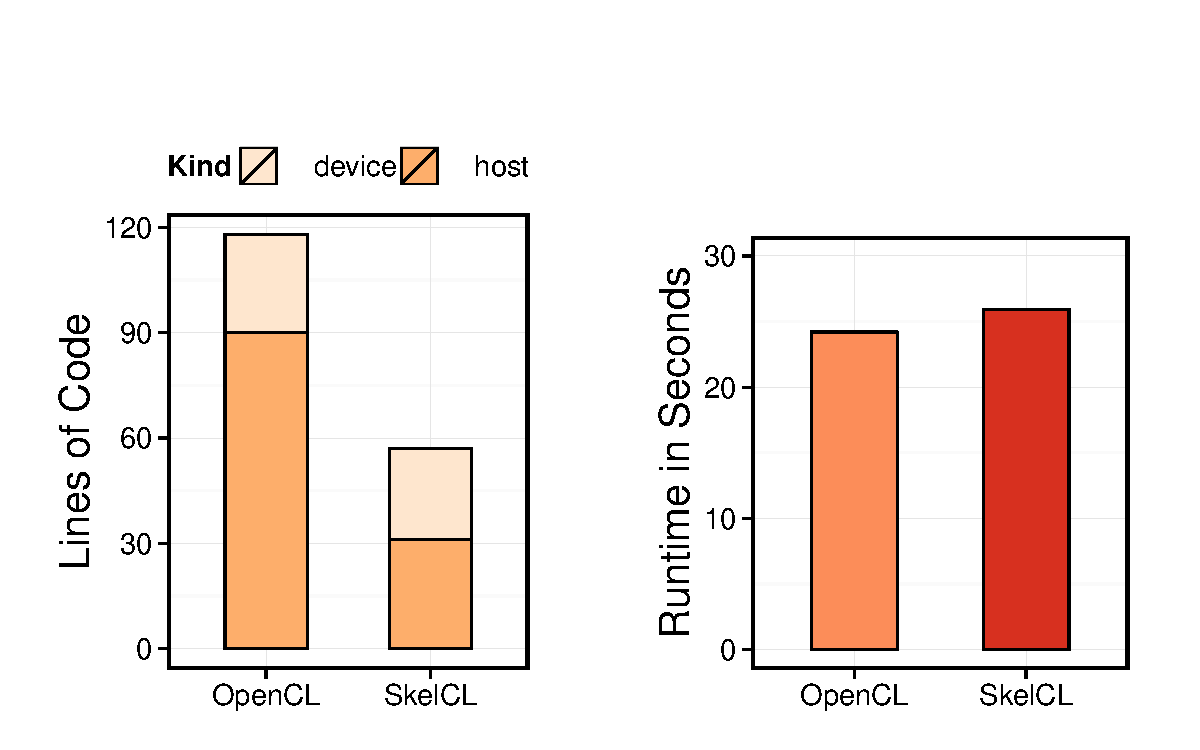
\includegraphics[width=.75\textwidth]{mandelbrot}
  \caption{Visualization of a part of the Mandelbrot set. The image was produced using the \SkelCL library.}
  \label{fig:mandelbrot}
\end{figure}

The Mandelbrot~\cite{Mandelbrot1980} set includes all complex numbers $c \in {\mathbb C}$ for which the sequence
\begin{equation}
	z_{i+1} = z_{i}^{2} + c,\qquad i\in {\mathbb N}
	\label{eq:mandelbrot}
\end{equation}
starting with $z_{0}=0$ does not escape to infinity.
When drawn as an image with each pixel representing a complex number, the boundary of the Mandelbrot set forms a fractal.
\autoref{fig:mandelbrot} shows an image visualizing part of the Mandelbrot set.
The software producing the image was implemented using the \SkelCL library. 
The calculation of such an image is a time-consuming task, because the sequence given by~\autoref{eq:mandelbrot} has to be calculated for every pixel.
If this sequence does not cross a given threshold for a given number of iteration steps, it is presumed that the sequence will converge.
The respective pixel is thus taken as a member of the Mandelbrot set, and it is displayed black.
Other pixels outside are assigned a color that corresponds to the number of iterations of the sequence given by~\autoref{eq:mandelbrot}.
Computing a Mandelbrot fractal is easily parallelizable, as all pixels of the fractal can be computed simultaneously.

\subsubsection*{\SkelCL Implementation}
\label{sec:mandelbrot:implementation}
The \SkelCL implementation of the Mandelbrot set computations uses the \map skeleton as shown in \autoref{eq:skelcl:mandelbrot}.
\begin{align}
  mandelbrot\ w\ h =&  \nonumber\\
         map\ compute&ColorOfPixel\ (generateIndex\ w\ h)
  \label{eq:skelcl:mandelbrot}
\end{align}
\todo{Explain $generateIndex$ and connection to \ref{eq:mandelbrot}}
Here function $mandelbrot$ is defined taking two arguments -- the width $w$ and height $h$ of the image to compute.
The function is defined in terms of the \map skeleton customized with $computeColorOfPixel$ computing the color of a single pixel of the image (not shown here) and operating on an input matrix of size $w\times h$ consisting of indices.

The implementation using the \SkelCL library is shown in \autoref{lst:skelcl:mandelbrot}.
A user-defined data type is introduced to represent the color of a pixel (line~\ref{lst:skelcl:mandelbrot:pixel}).
An instance of the \map skeleton is created in line~\ref{lst:skelcl:mandelbrot:map} and applied to \code{IndexMatrix} (line~\ref{lst:skelcl:mandelbrot:apply}).
The \code{IndexMatrix} represents all indices up to a given width and height.
It is implemented as a special representation of the generic \code{Matrix} class to avoid explicitly storing the indices in memory.
Instead when accessing an element the index value is computed on the fly.
This implementation avoids allocation of memory for storing the indices and transferring them to the \GPU.


\begin{lstlisting}[%                                                             
caption={Implementation of the Mandelbrot set computation in \SkelCL},%
numbers=left,%
float=tb,
label={lst:skelcl:mandelbrot}]
typedef struct { char r; char g; char b; } Pixel;$\label{lst:skelcl:mandelbrot:pixel}$

Pixel computeColorOfPixel(IndexPoint) { ... };

void mandelbrot(const int width, const int height) {
  auto m = map(computeColorOfPixel);$\label{lst:skelcl:mandelbrot:map}$
  auto image = m(IndexMatrix{w, h});$\label{lst:skelcl:mandelbrot:apply}$
  writeToDisk(image); }
\end{lstlisting}

We created two similar parallel implementations for computing a Mandelbrot fractal using CUDA and OpenCL.\todo{Show in appendix?}
We compare the programming effort and performance for these implementations against our \SkelCL implementation.

\subsubsection*{Programming effort}
\label{sec:mandelbrot:programming}

CUDA and \SkelCL require a single line of code for initialization in the host code, whereas OpenCL requires a lengthy initialization of different data structures which takes about 20 lines of code.

The host code differs significantly between all implementations.
In CUDA, the kernel is called like an ordinary function.
A proprietary syntax is used to specify the size of work-groups executing the kernel.
With OpenCL, several API functions are called to load and build the kernel, pass arguments to it and to launch it using a specified work-group size.
In \SkelCL, the \map skeleton is used to compute the color of all pixels in the image.
An \code{IndexMatrix} representing complex numbers, each of which is processed to produce a pixel of the Mandelbrot fractal, is passed to the \map skeleton upon execution.
Specifying the work-group size is mandatory in CUDA and OpenCL, whereas this is optional in \SkelCL.

\paragraph{Program size}
The OpenCL-based implementation has 118 lines of code (kernel: 28~lines, host program: 90~lines) and is thus more than twice as long as the CUDA and \SkelCL versions with 49 lines (28, 21) and 57 lines (26, 31), respectively (see \autoref{fig:mandelbrot_runtime}).
The lengths of the CUDA- and \SkelCL-based implementations differ by only a few lines.

\paragraph{Kernel size}
The kernel function is similar in all implementations: it takes a pixel's position (\ie, a complex number) as input, performs the iterative calculation for this pixel, and returns the pixel's color.
However, while the input positions are given explicitly when using the \map skeleton in SkelCL, no positions are passed to the kernel in the CUDA- and OpenCL-based implementations.
The positions are implicitly determined based on the work-item's index.

\subsubsection*{Performance experiments}
\label{sec:mandelbrot:performance}
\todo{Exclude CUDA ?}

\begin{figure}[tb]
    \centering
    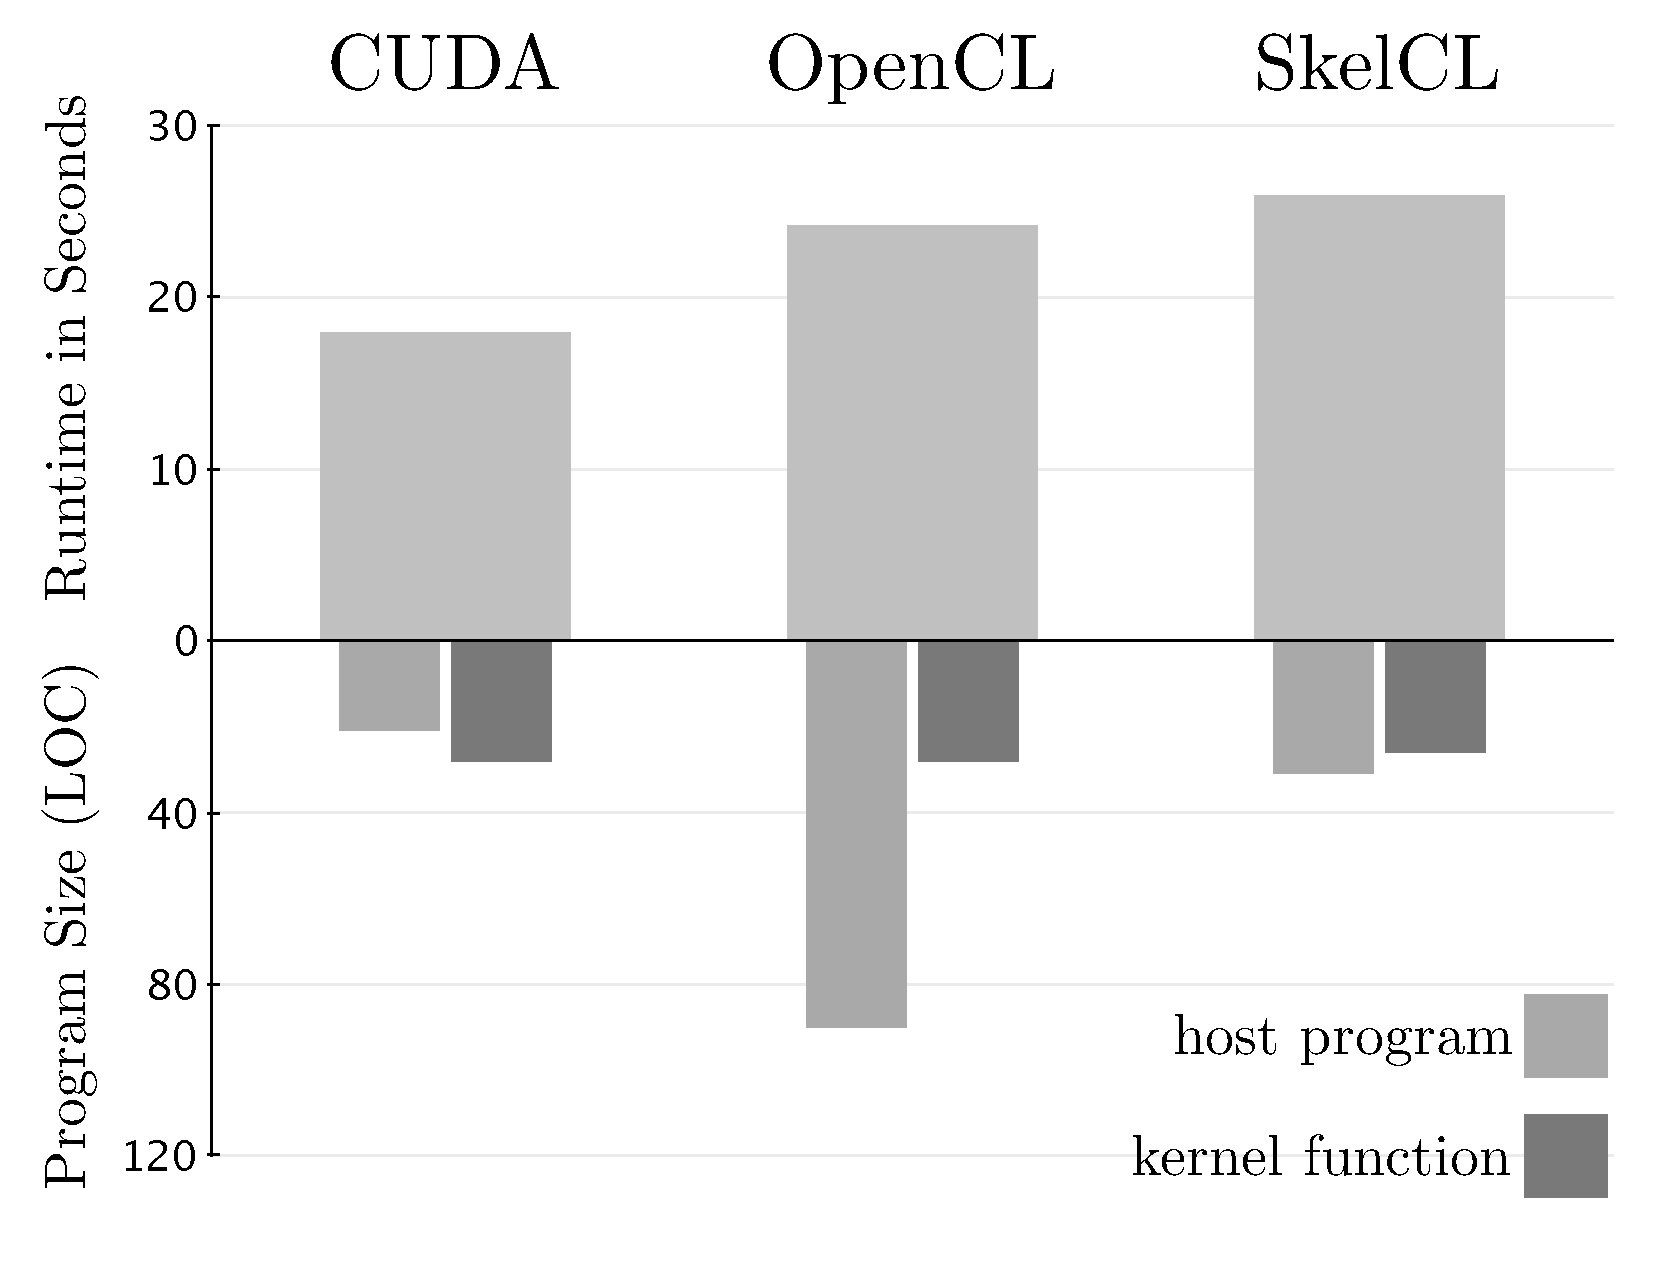
\includegraphics[width=0.6\textwidth]{HIPS/ChartMandelbrot}
    \caption{Runtime and program size of the Mandelbrot application.}
    \label{fig:mandelbrot_runtime}
\end{figure}%


We tested our implementations on a single \GPU of our test system to compute a Mandelbrot fractal of size 4096$\times$3072 pixels.
In CUDA and OpenCL, work-groups of 16$\times$16 are used; \SkelCL uses its default work-group size of~256 work-items.

The results are shown in \autoref{fig:mandelbrot_runtime}.
As compared to the runtime of the \SkelCL-based implementation (26 seconds), the implementation based on OpenCL (25 seconds) and CUDA (18 seconds) are faster by 4\% and 31\%, respectively.
Since \SkelCL is built on top of OpenCL, the performance difference of \SkelCL and OpenCL can be regarded as the overhead introduced by SkelCL.
Previous work~\cite{KongDiYaLiCaStMaZh2010} also reported that CUDA was usually faster than OpenCL, which also explains the higher performance of the implementation based on CUDA.
The Mandelbrot application demonstrates that \SkelCL introduces a tolerable overhead of less than 5\% as compared to OpenCL.
A clear benefit of this overhead is the reduced programming effort required by the SkelCL program.



\section{Linear Algebra Applications}

BLAS ... important building blocks ...
\todo{Write stuff}

\subsection{Sum of absolute values}
\label{sec:asum}
\autoref{eq:asum} shows the mathematical definition of the sum of absolute values (short \emph{asum}) for a vector $\vec{x}$ of length $n$ with elements $x_i$:
\begin{equation}
  asum\ \vec{x} = \sum_{i=0}^{n} | x_i |
  \label{eq:asum}
\end{equation}
For all elements of the vector the absolute values are added up to produce the final scalar result.

\subsubsection*{\SkelCL Implementation}
In the \SkelCL programming model we can express \emph{asum} using the \map and \reduce skeletons as follows:
\begin{align}
  asum\ \vec{x} &= reduce\ (+)\ 0\ \big(\ map\ (|\, .\, |)\ \vec{x}\ \big)\label{eq:asum:skelcl}\\
  \text{where:} \qquad | a | &=
    \left\{
      \begin{array}{r l}
      a & \text{if } a \geq 0\\
      -a & \text{if } a < 0
      \end{array}
    \right.\nonumber
\end{align}

The \map skeleton applies the $abs$ function to each element of the input vector before the \reduce skeleton is used to sum up the elements.

The implementation using the \SkelCL library is shown in \autoref{lst:skelcl:asum}.
In lines~\ref{lst:skelcl:asum:skeletons:start}--\ref{lst:skelcl:asum:skeletons:end} the customized skeletons are defined.
The \map skeleton in \autoref{eq:asum:skelcl} corresponds directly to lines~\ref{lst:skelcl:asum:skeletons:start} and~\ref{lst:skelcl:asum:abs} in \autoref{lst:skelcl:asum} where the $|\, .\, |$ function is represented using a \Cpp lambda expression.
Line~\ref{lst:skelcl:asum:skeletons:end} corresponds directly to the \reduce skeleton in \autoref{eq:asum:skelcl}.
By applying the skeletons to the input vector (line~\ref{lst:skelcl:asum:call}) the result is computed and accessed in line~\ref{lst:skelcl:asum:return}.
In the \SkelCL library implementation the \reduce skeleton returns a vector containing a single element.
The containers in the \SkelCL library are implemented as \emph{futures}~\cite{HewittBa1977,FriedmanWi1978}.
This allows the computation of all skeletons to be performed asynchronously, \ie, when executing a skeleton the computation is launched and the called function returns immediately.
When accessing values of the returned container, \eg, via the array subscript operator as shown in line~\ref{lst:skelcl:asum:return}, the call will block until the accessed value has been computed.

\begin{lstlisting}[%                                                             
caption={Implementation of the \emph{asum} application in \SkelCL},%
numbers=left,%
float=tb,
label={lst:skelcl:asum}]
float asum(const Vector<float>& x) {
  auto absAll = map($\label{lst:skelcl:asum:skeletons:start}$
      [](float a){ if (a >= 0) return a; else return -a; });$\label{lst:skelcl:asum:abs}$
  auto sumUp = reduce([](float a, float b){return a+b;}, 0);$\label{lst:skelcl:asum:skeletons:end}$
  auto result = sumUp( absAll( x ) );$\label{lst:skelcl:asum:call}$
  return result[0]; }$\label{lst:skelcl:asum:return}$
\end{lstlisting}

We compare this implementation against a native OpenCL implementation and an implementation using the CUBLAS library.

\subsubsection*{Programming effort}
\todo{...}

\subsubsection*{Performance experiments}
\todo{...}

As discussed in \autoref{chapter:skelcl} the \SkelCL library implementation generates one (or more) OpenCL kernel for each skeleton.
This procedure makes it difficult to \emph{merge} multiple OpenCL kernels into a single one, which would be required to achieve a competitive performance to the native OpenCL implementation.
In \autoref{ch:fifth}, we will discuss a novel compilation technique addressing this challenge.
This technique supports the generation of a single efficient OpenCL kernel, also for implementing applications like the \emph{asum} example.

\subsection{Dot product}
\label{sec:dot}
The computation of the dot product, \aka scalar product, is a common mathematical operation performed on two input vectors $\vec{x}$ and $\vec{y}$ of identical length $n$ as defined in \autoref{eq:dot_product}:
\begin{equation}
  dotProduct\ \vec{x}\ \vec{y} = \sum_{i=0}^{n} x_i \times y_i
  \label{eq:dot_product}
\end{equation}

\subsubsection*{\SkelCL Implementation}
In \SkelCL we can express $dotProduct$ using the \zip and \reduce skeletons as follows:
\begin{equation}
  dotProduct\ \vec{x}\ \vec{y} = reduce\ (+)\ 0\ \big(\ zip\ (\times)\ \vec{x}\ \vec{y}\ \big)
\end{equation}

The \zip skeleton performs the pairwise multiplication of the input vectors before the \reduce skeleton is used to sum up the intermediate results.

\autoref{lst:skelcl:dot} shows the implementation using the \SkelCL library.
The structure of the implementation is very similar to the \emph{asum} application discussed in \autoref{sec:asum}.
Here we use the \code{front} member function to access the first (and only) element of the computed result vector.

\begin{lstlisting}[%                                                             
caption={Implementation of the dot product application in \SkelCL},%
numbers=left,%
float=tb,
label={lst:skelcl:dot}]
float dotProduct(const Vector<float>& x,
                 const Vector<float>& y) {
  auto mult  = zip([](float x, float y){return x*y;});$\label{lst:skelcl:dot:skeletons:start}$
  auto sumUp = reduce([](float x, float y){return x+y;}, 0);$\label{lst:skelcl:dot:skeletons:end}$
  return sumUp( mult( x, y ) ).front(); }$\label{lst:skelcl:dot:call}$
\end{lstlisting}

\subsubsection*{Programming effort}
\todo{...}

\subsubsection*{Performance experiments}
\todo{...}

\subsection{Matrix Multiplication}

The multiplication of matrices is a basic operation in linear algebra and, therefore, a fundamental building block for many scientific applications.
An $n\times d$ matrix $A$ is multiplied with a $d\times m$ matrix $B$ to produce an $n\times m$ matrix $C$, where the elements of $C$ are computed as:
\begin{equation*}
  C_{ij} = \sum_{k=0}^{d} A_{ik} \times B_{kj}, \qquad \forall\ i \in 1, \ldots, n \wedge j \in 1, \ldots, m
\end{equation*}
Here $A_{i*}$ refers to the $i$th row of $A$ and $B_{*j}$ to the $j$th column of $B$.
\autoref{fig:mm} visualizes this computation.
To compute the highlighted element in matrix $C$, the highlighted row of matrix $A$ is combined with the highlighted column of matrix $B$.
For computing the entire matrix $C$, \emph{all pairs} of rows from $A$ and columns of $B$ have to be processed.
Therefore, in \SkelCL the \allpairs skeleton can be used to express matrix multiplication.

\begin{figure}[tb]
  \centering
  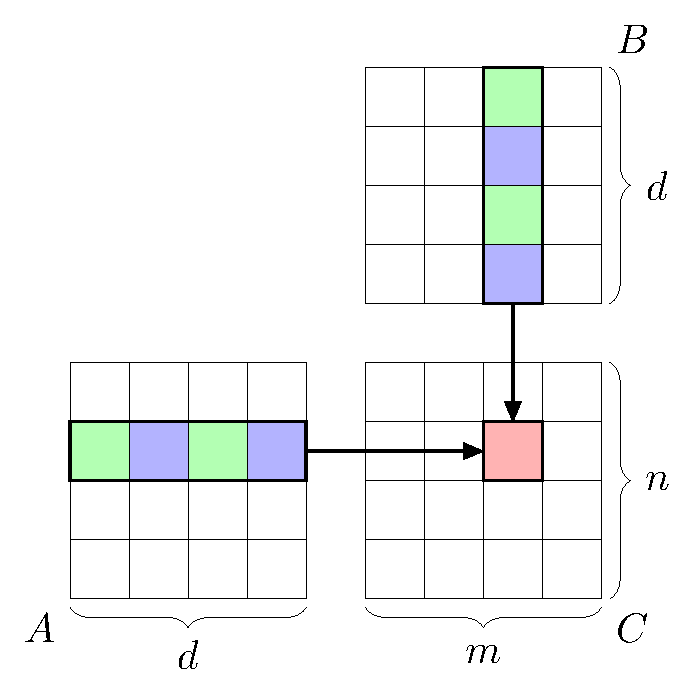
\includegraphics[width=0.5\textwidth]{HLPP/mm}
  \caption[Visalization of matrix multiplication.]%
          {Matrix multiplication $A\times B = C$.
           The red highlighted element in matrix $C$ is computed by combining the highlighted row of matrix $A$ with the highlighted column of matrix $B$.}
  \label{fig:mm}
\end{figure}


\subsubsection*{\SkelCL Implementation}
\autoref{eq:skelcl:mm} shows how matrix multiplication can be expressed using the \allpairs skeleton in \SkelCL:
\begin{align}
  \label{eq:skelcl:mm}
  mm\ A\ B &= allpairs\ f\ A\ B^T\\
  \text{where:} \qquad f\ \vec{a}\ \vec{b} &= \sum_{k=0}^d a_k \times b_k \nonumber
\end{align}
When looking back at \autoref{sec:dot}, we can see, that $f$ is actually the dot product computation, therefore, we can write:
\begin{align}
  mm\ A\ B &= allpairs\ dotProduct\ A\ B^T
  \label{eq:skelcl:mm:dot}
\end{align}
We know that we can express the dot product as a sequential composition of the \zip and \reduce skeletons.
In \autoref{section:skelcl-programming-model:specialSkeletons} we discussed a specialized implementation of the \allpairs skeleton for computations which can be expressed in this way.
Therefore, we can use the \SkelCL library to develop two implementations:
1) using the generic \allpairs skeleton; and 2) using the specialized \allpairs skeleton.

\autoref{lst:skelcl:mm:generic} shows the implementation of matrix multiplication using the generic \allpairs skeleton.
\begin{lstlisting}[%                                                             
caption={Implementation of matrix multiplication using the generic \allpairs skeleton in \SkelCL.},%
numbers=left,%
float=tb,
label={lst:skelcl:mm:generic}]
Matrix<float> mm(const Matrix<float>& A,$\label{lst:skelcl:mm:generic:CPU:start}$
                 const Matrix<float>& B) {
  skelcl::init();
  auto mm = allpairs($\label{lst:skelcl:mm:generic:CPU:stop}$
    [](const Vector<float>& a, const Vector<float>& b) {$\label{lst:skelcl:mm:generic:GPU:start}$
      float c = 0.0f;
      for (int i = 0; i < a.size(); ++i)
        c += a[i] * b[i];
      return c; });$\label{lst:skelcl:mm:generic:GPU:stop}$
  return mm(A, B); }$\label{lst:skelcl:mm:generic:CPU:call}$
\end{lstlisting}
The skeleton is customized with a lambda expression processing two vectors:
$a$ is a row vector of matrix $A$ and $b$ is a column vector of matrix $B$.
In this generic implementation the dot product computation is implemented using a \code{for} loop iterating over the vectors, multiplying elements pairwise and summing them up in the accumulation variable $c$.

\autoref{lst:skelcl:mm:special} shows the implementation of matrix multiplication using the specialized \allpairs skeleton.
\begin{lstlisting}[%                                                             
caption={Implementation of matrix multiplication using the specialized \allpairs skeleton in \SkelCL.},%
float=tb,%                                                                       
numbers=left,%
label={lst:skelcl:mm:special}]
Matrix<float> mm(const Matrix<float>& A,
                 const Matrix<float>& B) {
  skelcl::init();
  auto mult  = zipVector($\label{lst:skelcl:mm:special:zip}$
      [](float x, float y){return x*y;});$\label{lst:skelcl:mm:special:zipGPU}$
  auto sumUp = reduce($\label{lst:skelcl:mm:special:reduce}$
      [](float x, float y){return x+y;}, 0);$\label{lst:skelcl:mm:special:reduceGPU}$
  auto mm    = allpairs(sumUp, mult);
  return mm(A, B); }
\end{lstlisting}
Here the \allpairs skeleton is customized with \zip and \reduce skeletons defined in lines~\ref{lst:skelcl:mm:special:zip} and~\ref{lst:skelcl:mm:special:reduce}.
This implementation corresponds more closely to \autoref{eq:skelcl:mm:dot}:
as we express the dot product using these two skeletons (as shown in \autoref{sec:dot}).
Therefore, we reuse the definitions of \code{mult} and \code{sumUp} as used in \autoref{lst:skelcl:dot}.

\subsubsection*{Implementations used for comparison}
We compare six different implementations of matrix multiplication:
\begin{enumerate}
  \item the OpenCL implementation from~\cite{KirkHw2010} without optimizations,
  \item the optimized OpenCL implementation from~\cite{KirkHw2010} using \GPU local memory,
  \item the optimized BLAS implementation by AMD~\cite{APPML} written in OpenCL,
  \item the optimized BLAS implementation by Nvidia~\cite{cuBLAS} written in CUDA,
  \item the \SkelCL implementation in~\autoref{lst:skelcl:mm:generic} using the generic \allpairs skeleton,
  \item the \SkelCL implementation in~\autoref{lst:skelcl:mm:special} using the specialized \allpairs skeleton.
\end{enumerate}

\paragraph{1. OpenCL implementation}
The kernel of the first, unoptimized OpenCL implementation from~\cite{KirkHw2010} is shown in \autoref{lst:naive_opencl}.
\begin{lstlisting}[%                                                             
caption={[\OpenCL kernel of matrix multiplication without optimizations.]\OpenCL kernel of matrix multiplication without optimizations~\cite{KirkHw2010}.},%
float=tb,%
numbers=left,%
label={lst:naive_opencl}]
kernel void mm(global float* A, global float* B,
               global float* C, int m, int d, int n) {
  int row = get_global_id(0); int col = get_global_id(1);
  float sum = 0.0f;
  for (int k = 0; k < d; k++)
    sum += A[row * d + k] * B[k * n + col];
  C[row * n + col] = sum; }
\end{lstlisting}

\vspace{-.5em}
\paragraph{2. Optimized OpenCL implementations}
The kernel of the optimized OpenCL implementation from~\cite{KirkHw2010} using local memory is shown in \autoref{lst:local_mem_opencl}.
\begin{lstlisting}[%                                                             
caption={[\OpenCL kernel of the optimized matrix multiplication usgin local memory.]\OpenCL kernel of the optimized matrix multiplication using local memory~\cite{KirkHw2010}.},%
float=tb,%
numbers=left,%
label={lst:local_mem_opencl}]
#define T_WIDTH 16
kernel void mm(global float* A, global float* B,
               global float* C, int m, int d, int n) {
  local float Al[T_WIDTH][T_WIDTH];$\label{lst:local_mem_opencl:allocA}$
  local float Bl[T_WIDTH][T_WIDTH];$\label{lst:local_mem_opencl:allocB}$
  int row = get_global_id(0); int col = get_global_id(1);
  int l_row = get_local_id(0);  int l_col = get_local_id(1);
  float sum = 0.0f;
  for (int m = 0; m < d / T_WIDTH; ++m {$\label{lst:local_mem_opencl:loop}$
    Al[l_row][l_col] = A[row * d + (m * T_WIDTH + l_col)];$\label{lst:local_mem_opencl:loadA}$
    Bl[l_row][l_col] = B[(m * T_WIDTH + l_row) * d + col];$\label{lst:local_mem_opencl:loadB}$
    barrier(CLK_LOCAL_MEM_FENCE);$\label{lst:local_mem_opencl:barrier1}$
    for (int k = 0; k < T_WIDTH; k++)
      sum += Al[l_row][k] * Bl[k][l_col];$\label{lst:local_mem_opencl:comp}$
    barrier(CLK_LOCAL_MEM_FENCE); }$\label{lst:local_mem_opencl:barrier2}$
  C[row * n + col] = sum; }
\end{lstlisting}
Two fixed-sized arrays of local memory are allocated in lines~\ref{lst:local_mem_opencl:allocA} and~\ref{lst:local_mem_opencl:allocB}.
Matrix multiplication is carried out in the loop starting in line~\ref{lst:local_mem_opencl:loop}.
In each iteration, data is loaded into the local memory (lines~\ref{lst:local_mem_opencl:loadA} and~\ref{lst:local_mem_opencl:loadB}) before it is used in the computation in line~\ref{lst:local_mem_opencl:comp}.
Note that two synchronization barriers are required (lines~\ref{lst:local_mem_opencl:barrier1} and~\ref{lst:local_mem_opencl:barrier2}) to ensure that the data is fully loaded into the local memory and that the data is not overwritten while other work-items are still using it.

Both OpenCL implementations 1. and 2. from~\cite{KirkHw2010} are restrictive:
they are only capable of performing matrix multiplication for square matrices.

\vspace{-.5em}
\paragraph{3. BLAS implementation by AMD}
The implementation offered by AMD is called clBLAS, written in OpenCL and is part of their Accelerated Parallel Processing Math Libraries (APPML)~\cite{APPML}.

\vspace{-.5em}
\paragraph{4. BLAS implementation by NVIDIA}
The cuBLAS~\cite{cuBLAS} is implemented using CUDA and, therefore, can only be used on GPUs built by NVIDIA.

\subsubsection*{Programming effort}
\autoref{fig:mat_mult_loc} shows the comparison regarding the number of lines of code (LoCs) required for each of the six implementations.
\autoref{tab:mat_mult_loc} presents the detailed numbers.
We did not count those LoCs which are not relevant for parallelization and are similar in all six implementations, like initializing the input matrices with data and checking the result for correctness.
For every implementation, we distinguish between \CPU (host) code and \GPU (kernel) code.

In the \OpenCL implementations, the \GPU code includes the kernel definition, as shown in \autoref{lst:naive_opencl} and \autoref{lst:local_mem_opencl};
the \CPU code includes the initialization of \OpenCL, memory allocations, explicit data transfer operations, and management of the execution of the kernel.

In the BLAS implementations, the \CPU code contains the initialization of the corresponding BLAS library, memory allocations, as well as a library call for performing the matrix multiplication;
no separate definition of \GPU code is necessary, as the \GPU code is defined inside the library function calls.

For the implementation based on the generic \allpairs skeleton (\autoref{lst:skelcl:mm:generic}), we count lines~\ref{lst:skelcl:mm:generic:CPU:start}--\ref{lst:skelcl:mm:generic:CPU:stop} and~\ref{lst:skelcl:mm:generic:CPU:call} as the \CPU code, and the definition of the customizing function in lines~\ref{lst:skelcl:mm:generic:GPU:start}--\ref{lst:skelcl:mm:generic:GPU:stop} as the \GPU code.
For the implementation based on the specialized \allpairs skeleton (\autoref{lst:skelcl:mm:special}), lines~\ref{lst:skelcl:mm:special:zipGPU} and~\ref{lst:skelcl:mm:special:reduceGPU} are the \GPU code, while all other lines constitute the \CPU code.

Both skeleton-based implementations are clearly the shortest, with 10 and 9 LoCs.
The next shortest implementation is the cuBLAS implementation with 65 LoCs -- 7 times longer than the \SkelCL-based implementations.
The other three implementations using \OpenCL require even 9 times more LoCs than the \SkelCL-based implementations.

Besides their length, the \OpenCL-based implementations require the application developer to explicitly implement many low-level, error-prone tasks, like dealing with pointers and offset calculations.
Furthermore, the skeleton-based implementations are more general, as they can be used for arbitrary allpairs computations, while all \OpenCL-based implementations can compute matrix multiplication only.

\begin{figure}[tb]
  \centering
  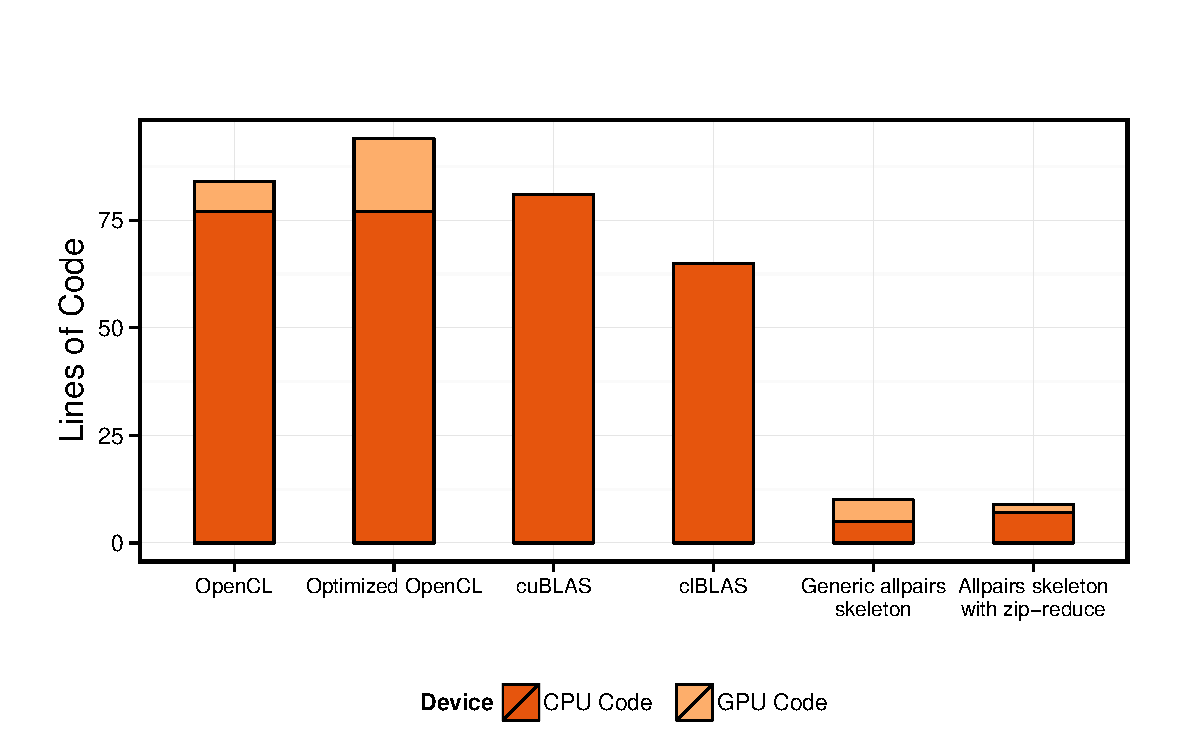
\includegraphics[width=0.9\textwidth]{HLPP/mat_mult_loc}
  \caption[Programming effort of four \OpenCL-based and two \SkelCL-based matrix multiplication implementations.]%
          {Programming effort (Lines of Code) of four \OpenCL-based vs. two \SkelCL-based implementations.}
  \label{fig:mat_mult_loc}
\end{figure}
\begin{table}[tb]
  \centering
  \begin{tabular}{lrr}
    \toprule
              & \multicolumn{2}{c}{Lines of Code} \\
    \cmidrule(r){2-3}
    Implementation & \CPU & \GPU \\
    \midrule
    \OpenCL           & 77 &  7 \\
    Optimized \OpenCL & 71 & 17 \\
    cuBLAS            & 81 & -- \\
    clBLAS            & 65 & -- \\
    Generic \allpairs  & \multirow{2}{*}{5} & \multirow{2}{*}{5}\\
    skeleton\\
    Specialized \allpairs & \multirow{2}{*}{7} & \multirow{2}{*}{2}\\
    skeleton\\
    \bottomrule
  \end{tabular}
  \caption[Lines of Code of matrix multiplication of all compared implementaitons.]%
          {Lines of Code of all compared implementations.}
  \label{tab:mat_mult_loc}
\end{table}

\subsubsection*{Performance experiments}
We performed our experiments with the six different implementations 1. -- 6. of matrix multiplication on two different computer systems with GPUs:
\begin{itemize}[leftmargin=50pt]
  \item[System A:] Our general testing system already described in~\autoref{sec:skelcl:experimental_setup}:
    an NVIDIA S1070 equipped with four Nvidia Tesla \GPUs, each with 240 streaming processors and 4 GByte memory.
  \item[System B:] An AMD Radeon HD 6990 graphics card containing two \GPUs, each with 1536 streaming processors and 1 GByte memory.
\end{itemize}

\begin{figure}[tb]
  \centering
  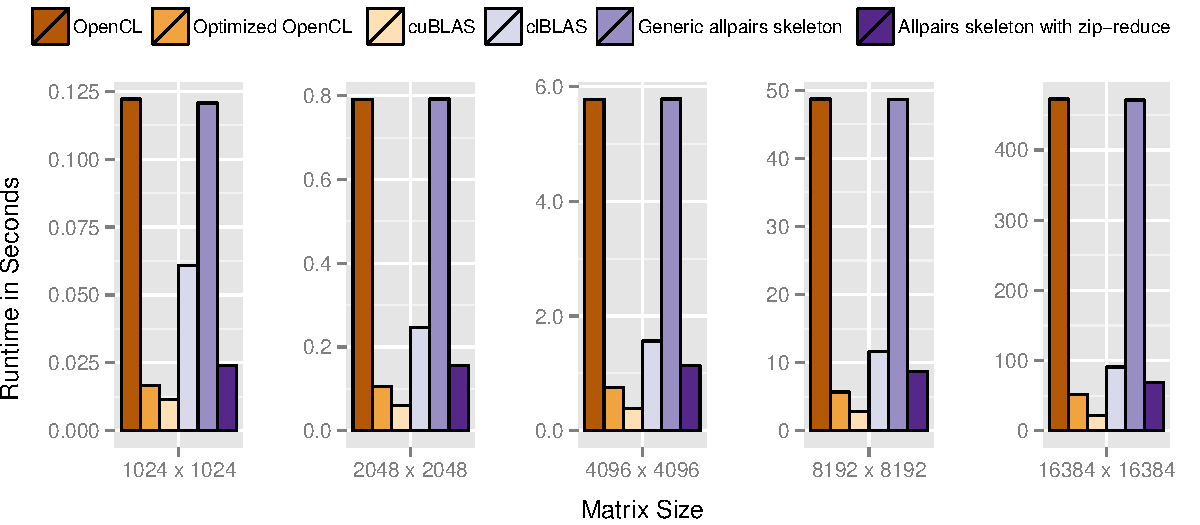
\includegraphics[width=0.9\textwidth]{HLPP/mat_mult_sizes}
  \caption[Runtime of different matrix multiplication implementations on an NVIDIA system.]%
          {Runtime of different matrix multiplication implementations on the NVIDIA system for different sizes of the matrices.}
  \label{fig:mat_mult_single}
\end{figure}
\begin{table}[tb]
  \centering
  \begin{tabular}{lrrrrr}
    \toprule
              & \multicolumn{5}{c}{Runtimes in Seconds} \\
    \cmidrule(r){2-6}
    \multirow{2}{*}{Implementation} & $1024$ & $2048$ & $4096$ & $8192$ & $16384$ \\
                                    & $\times 1024$ & $\times 2048$ & $\times 4096$ & $\times 8192$ & $\times 16384$\\
    \midrule
    \OpenCL            & 0.122 & 0.791 & 5.778 & 48.682 & 472.557 \\
    Optimized \OpenCL  & 0.017 & 0.105 & 0.752 &  5.683 &  51.337 \\
    cuBLAS             & 0.012 & 0.059 & 0.387 &  2.863 &  22.067 \\
    clBLAS             & 0.061 & 0.246 & 1.564 & 11.615 &  90.705 \\
    Generic \allpairs  & \multirow{2}{*}{0.121} & \multirow{2}{*}{0.792} & \multirow{2}{*}{5.782} & \multirow{2}{*}{48.645} & \multirow{2}{*}{471.235} \\
    skeleton\\
    Specialized \allpairs & \multirow{2}{*}{0.024} & \multirow{2}{*}{0.156} & \multirow{2}{*}{1.134} & \multirow{2}{*}{8.742} & \multirow{2}{*}{68.544} \\
    skeleton\\
    \bottomrule
  \end{tabular}
  \caption[Runtime results for all tested implementations of matrix multiplication on an NVIDIA system.]
          {Runtime results for all tested implementations on the NVIDIA system.}
  \label{tab:mat_mult_single}
\end{table}

In all our experiments, we include the time of data transfers to and from the \GPU, \ie the measured runtime consists of:
1) uploading the two input matrices to the \GPU;
2) performing the actual matrix multiplication;
3) downloading the computed result matrix.

\paragraph{System A (one \GPU)}
\autoref{fig:mat_mult_single} shows the runtime in seconds of all six implementations for different sizes of the matrices (note that for readability reasons, all charts are scaled differently).
For detailed numbers, see \autoref{tab:mat_mult_single}.

Clearly, the naive \OpenCL-based implementation and the \SkelCL-based implementation using the generic \allpairs skeleton are the slowest, because both do not use the fast \GPU local memory, in contrast to all other implementations.

The \SkelCL-based implementation using the specialized \allpairs skeleton performs between 5.0 and 6.8 times faster than the implementation using the generic allpairs skeleton, but is 33\% slower on $16384\times 16384$ matrices than the optimized \OpenCL-based implementation using local memory.
However, the latter implementation can only be used for square matrices and, therefore, it benefits from omitting many conditional statements and boundary checks.

\begin{figure}[tb]
  \centering
  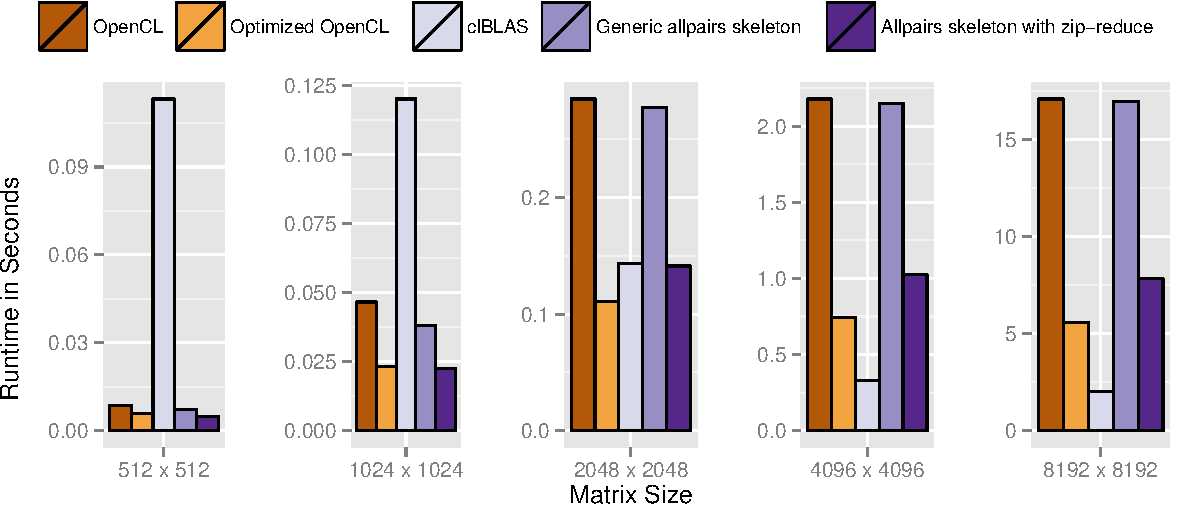
\includegraphics[width=0.9\textwidth]{HLPP/mat_mult_sizes_hd6990}
  \caption[Runtime of different matrix multiplication implementations on an AMD ststem.]%
          {Runtime of all compared implementations for a matrix multiplication on the AMD system using one \GPU.}
  \label{fig:mat_mult_single_amd}
\end{figure}
\begin{table}[b]
  \centering
  \begin{tabular}{lrrrrr}
    \toprule
              & \multicolumn{5}{c}{Runtimes in Seconds} \\
    \cmidrule(r){2-6}
    \multirow{2}{*}{Implementation} & $512$ & $1024$ & $2048$ & $4096$ & $8192$ \\
                                    & $\times 512$ & $\times 1024$ & $\times 2048$ & $\times 4096$ & $\times 8192$ \\
    \midrule
    \OpenCL            & 0.008 & 0.046 & 0.284 & 2.178 & 17.098 \\
    Optimized \OpenCL  & 0.006 & 0.023 & 0.111 & 0.743 &  5.569 \\
    clBLAS             & 0.113 & 0.120 & 0.143 & 0.329 &  2.029 \\
    Generic \allpairs  & \multirow{2}{*}{0.007} & \multirow{2}{*}{0.038} & \multirow{2}{*}{0.278} & \multirow{2}{*}{2.151} & \multirow{2}{*}{16.983} \\
    skeleton\\
    Specialized \allpairs & \multirow{2}{*}{0.005} & \multirow{2}{*}{0.023} & \multirow{2}{*}{0.141} & \multirow{2}{*}{1.025} & \multirow{2}{*}{7.842} \\
    skeleton\\
    \bottomrule
  \end{tabular}
  \caption[Runtime results for all tested implementations of matrix multiplication on an AMD system.]%
          {Runtime results for all tested implementations of matrix multiplication on the AMD system.}
  \label{tab:mat_mult_single_amd}
\end{table}

Not surprisingly, cuBLAS by Nvidia is the fastest of all implementations, as it is highly tuned specifically for Nvidia \GPUs using CUDA.
The clBLAS implementation by AMD using \OpenCL performs not as well:
presumably, it is optimized for AMD \GPUs and performs poorly on other hardware.
Our optimized \allpairs skeleton implementation outperforms the clBLAS implementation for all matrix sizes tested.

\paragraph{System B (one \GPU)}
\autoref{fig:mat_mult_single_amd} shows the measured runtime in seconds for five of the six implementations for different sizes of the matrices.
Detailed numbers can be found in \autoref{tab:mat_mult_single_amd}.
We could not use the Nvidia-specific cuBLAS implementation as it does not work on the AMD \GPU.

For bigger matrices, the slowest implementations are, again, the unoptimized \OpenCL implementation and the implementation using the generic \allpairs skeleton.

The optimized \OpenCL implementation and the specialized \allpairs skeleton perform similarly.
For matrices of size $8192\times 8192$, the optimized \OpenCL implementation is about 30\% faster.

The clBLAS implementation performs very poorly for small matrices, but is clearly the fastest implementation for bigger matrices.
Similar to the cuBLAS implementation on the Nvidia hardware, it is not surprising that the implementation by AMD performs very well on their own hardware.


\begin{figure}[tb]
  \centering
  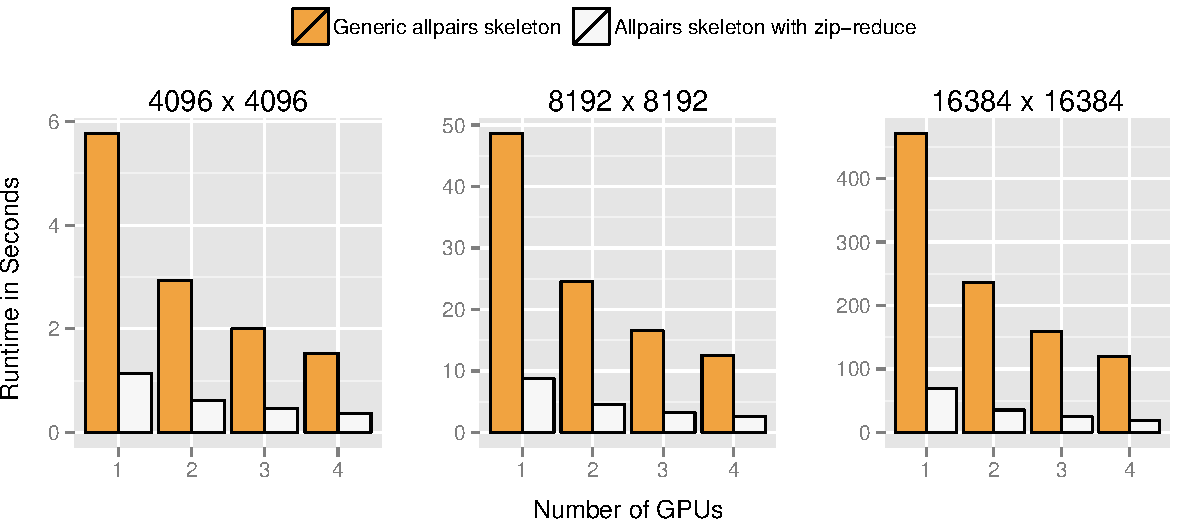
\includegraphics[width=0.9\textwidth]{HLPP/mat_mult_devices}
  \caption[Runtime of the \allpairs based matrix multiplication implementations using multiple \GPUs.]%
          {Runtime of the \allpairs based implementations using multiple \GPUs.}
  \label{fig:mat_mult_devices}
\end{figure}
\begin{table}[tb]
  \centering
  \begin{tabular}{llrrrcr}
    \toprule
              & & \multicolumn{3}{c}{Runtimes in Seconds} & & GFlops\\
    \cmidrule(r){3-5}
    \cmidrule(r){7-7}
    \multirow{2}{*}{Implementation}
     & Number    & $4096$ & $8192$ & $16384$ & & $16384$\\
     & of \GPUs   & $\times 4096$ & $\times 8192$ & $ \times 16384$ & & $ \times 16384$\\
    \midrule
    \multirow{4}{*}{\parbox[t]{2.3cm}{Generic \allpairs\\ skeleton}}
     & 1 \GPU  & 5.772 & 48.645 & 471.328 &&  18.72\\
     & 2 \GPUs & 2.940 & 24.495 & 236.628 &&  37.43\\
     & 3 \GPUs & 2.000 & 16.532 & 158.611 &&  56.17\\
     & 4 \GPUs & 1.527 & 12.540 & 119.786 &&  74.90\\[.5em]
    \multirow{4}{*}{\parbox[t]{2.3cm}{Specialized \allpairs\\ skeleton}}
     & 1 \GPU  & 1.137 &  8.740 &  68.573 && 130.93\\
     & 2 \GPUs & 0.613 &  4.588 &  35.294 && 262.18\\
     & 3 \GPUs & 0.461 &  3.254 &  24.447 && 392.87\\
     & 4 \GPUs & 0.368 &  2.602 &  19.198 && 523.91\\
    \bottomrule
  \end{tabular}
  \caption{Runtime of the allpairs based implementations of matrix multiplication using multiple \GPUs.
    For the matrices of size $16384\times 16384$ the results are also shown in GFlops.}
  \label{tab:mat_mult_devices}
\end{table}

\paragraph{System A (multiple \GPUs)}
\autoref{fig:mat_mult_devices} shows the runtime behavior for both \allpairs skeleton-based implementations when using up to four \GPUs of our multi-\GPU system.
The other four implementations are not able to handle multiple \GPUs and would have to be specially rewritten for such systems.
The newer version of Nvidia's cuBLAS implementation~\cite{} supports the execution on multiple \GPUs as well.
We observe a good scalability for both of our skeleton-based implementations, achieving speedups between 3.09 and 3.93 when using four \GPUs.
Detailed numbers can be found in \autoref{tab:mat_mult_devices}.
For the matrices of size $16384\times 16384$, performance is also provided in GFlops;
to compute this value we excluded the data-transfer time (as usually done in related work) for a better comparison.

\FloatBarrier




\section{Image Processing Applications}
\label{sec:imageProcessing}
Many image processing applications are inherently parallel as they often independently process the pixels of an image.
Common examples range from simple thresholding over noise reduction applications to techniques used in edge detection and pattern recognition~\cite{Umbaugh1997}.
In this section we will study three application examples from image processing and how they can be implemented using \SkelCL.

We start by looking at the Gaussian blur application which reduces noise in images and is often used as a preprocessing step in more complex algorithms.
We will then discuss two algorithms used for edge detection in images:
first, the Sobel edge detection application will be presented before, finally, the more complex Canny edge detection algorithm will be discussed.

All these three applications can be expressed using the \stencil skeleton but have different characteristics.
The Gaussian blur applies a single stencil computation, possibly iterated multiple times, for reducing the noise in images.
The Sobel edge detection applies a stencil computation once to detect edges in images.
The more advanced Canny edge detection algorithm consists of a sequence of stencil operations which are applied to obtain the final result.
For each application, we compare the performance of our two implementations of the \stencil skeletons: \code{MapOverlap} and \code{Stencil} with native OpenCL implementations using an input image of size $4096 \times 3072$.










\subsection{Gaussian blur}
\label{sec:gauss}
The Gaussian blur is a standard algorithm used in image processing~\cite{Umbaugh1997}.
One common application is reduction of image noise as shown in \autoref{fig:lena:noise}.
%
\begin{figure}[tb]
  \centering
  \begin{subfigure}[t]{.45\textwidth}
    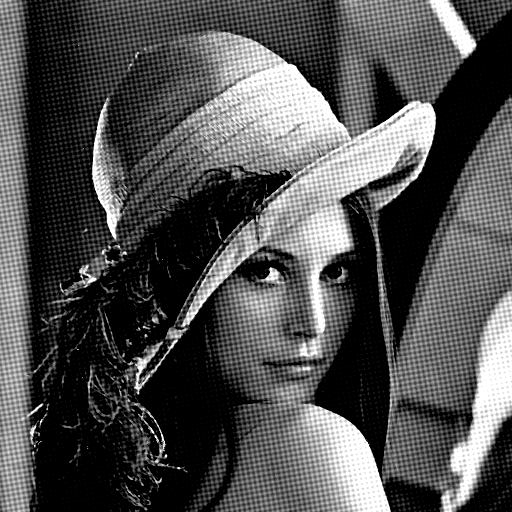
\includegraphics[width=\textwidth]{lenaNoise}
    \caption{Image with noise.}
    \label{fig:lena:noise:yes}
  \end{subfigure}
  \hfill
  \begin{subfigure}[t]{.45\textwidth}
    
\includegraphics[width=\textwidth]{lenaNoNoise}
    \caption{Image after applying the Gaussian blur.}
    \label{fig:lena:noise:no}
  \end{subfigure}
  \caption{Effect of applying the Gaussian blur to an noised image.}
  \label{fig:lena:noise}
\end{figure}
%
The image on the left has some noise as it is typically produced by halftone printing used to print newspapers.
The Gaussian blur has been applied to reduce the noise and produce the image on the right.

The Gaussian blur computes the color of every pixel using a weighted average of the neighboring pixel color values.
Using \SkelCL this application can easily be expressed using the \stencil skeleton.

\subsubsection*{\SkelCL Implementation}
\autoref{eq:gauss} shows the implementation in \SkelCL using the \stencil skeleton.
\begin{align}
  \label{eq:gauss}
  gauss&\ M = stencil\ f\ 1\ \overline{0}\ M \qquad\text{where:}\\
  &
  \begin{array}{ll}%
  f\ &\left[\begin{array}{lll}%
      \hspace{-.5em} M_{i-1,j-1}& \hspace{-.5em} M_{i-1,j} & \hspace{-.5em}M_{i-1,j+1}\vspace{-.25em}\\%
      \hspace{-.5em} M_{i,j-1}& \hspace{-.5em} M_{i,j} & \hspace{-.5em}M_{i,j+1}\vspace{-.25em}\\%
      \hspace{-.5em} M_{i+1,j-1}& \hspace{-.5em} M_{i+1,j} & \hspace{-.5em}M_{i+1,j+1}
    \end{array}\right]  = \\[2em]
          &\qquad \displaystyle\frac{\displaystyle\sum_{k=-1}^{1} \sum_{l=-1}^{1} (G\ k\ l)\cdot M_{i+k, j+k}}{9}
  \end{array} \nonumber\\[1em]
  &G\ x\ y = \frac{1}{2\pi \sigma^{2}} e^{-\frac{x^2 + y^2}{2\sigma^2}} \nonumber\\
  \text{and } \overline{0} \text{ is th}&\text{e constant function always returning 0.}\nonumber
\end{align}
$G$ is the two dimensional Gaussian function used in the customizing function $f$ to weight the neighboring values $M_{i,j}$.
The values gained from applying $G$ can be precomputed, as $G$ is only evaluated with values in the interval $[-1, 1]$ for $x$ and $y$.


\autoref{lst:skelcl:gauss} shows the implementation in the \SkelCL library of the Gaussian blur using the \code{MapOverlap} implementation of the \stencil skeleton.
Here the immediate neighboring pixels are access (lines~\ref{lst:skelcl:gauss:start}--\ref{lst:skelcl:gauss:end}) and used to compute a weighted value for each pixel.
The function performing the weighted sum is omitted here.
It is also possible to extend the \emph{range} of the Gaussian blur and include more neighboring pixel values in the computation.

\begin{lstlisting}[%                                                             
caption={Implementation of the Gaussian blur in \SkelCL using the \code{MapOverlap} implementation of the \stencil skeleton.},%
numbers=left,%
float=tb,
label={lst:skelcl:gauss}]
Matrix<char> gaussianBlur(const Matrix<char>& image) {
  auto gauss = mapOverlap(
    [](Neighborhood<char>& in) {
      char ul = in[{-1, -1}];$\label{lst:skelcl:gauss:start}$
      ...
      char lr = in[{+1, +1}];$\label{lst:skelcl:gauss:end}$
      return computeGaussianBlur(ul, ..., lr); },
    1, BorderHandling::NEUTRAL(0));
  return gauss(image); }
\end{lstlisting}

\subsubsection*{Programming effort}

\begin{figure}[tbp]
	\centering
	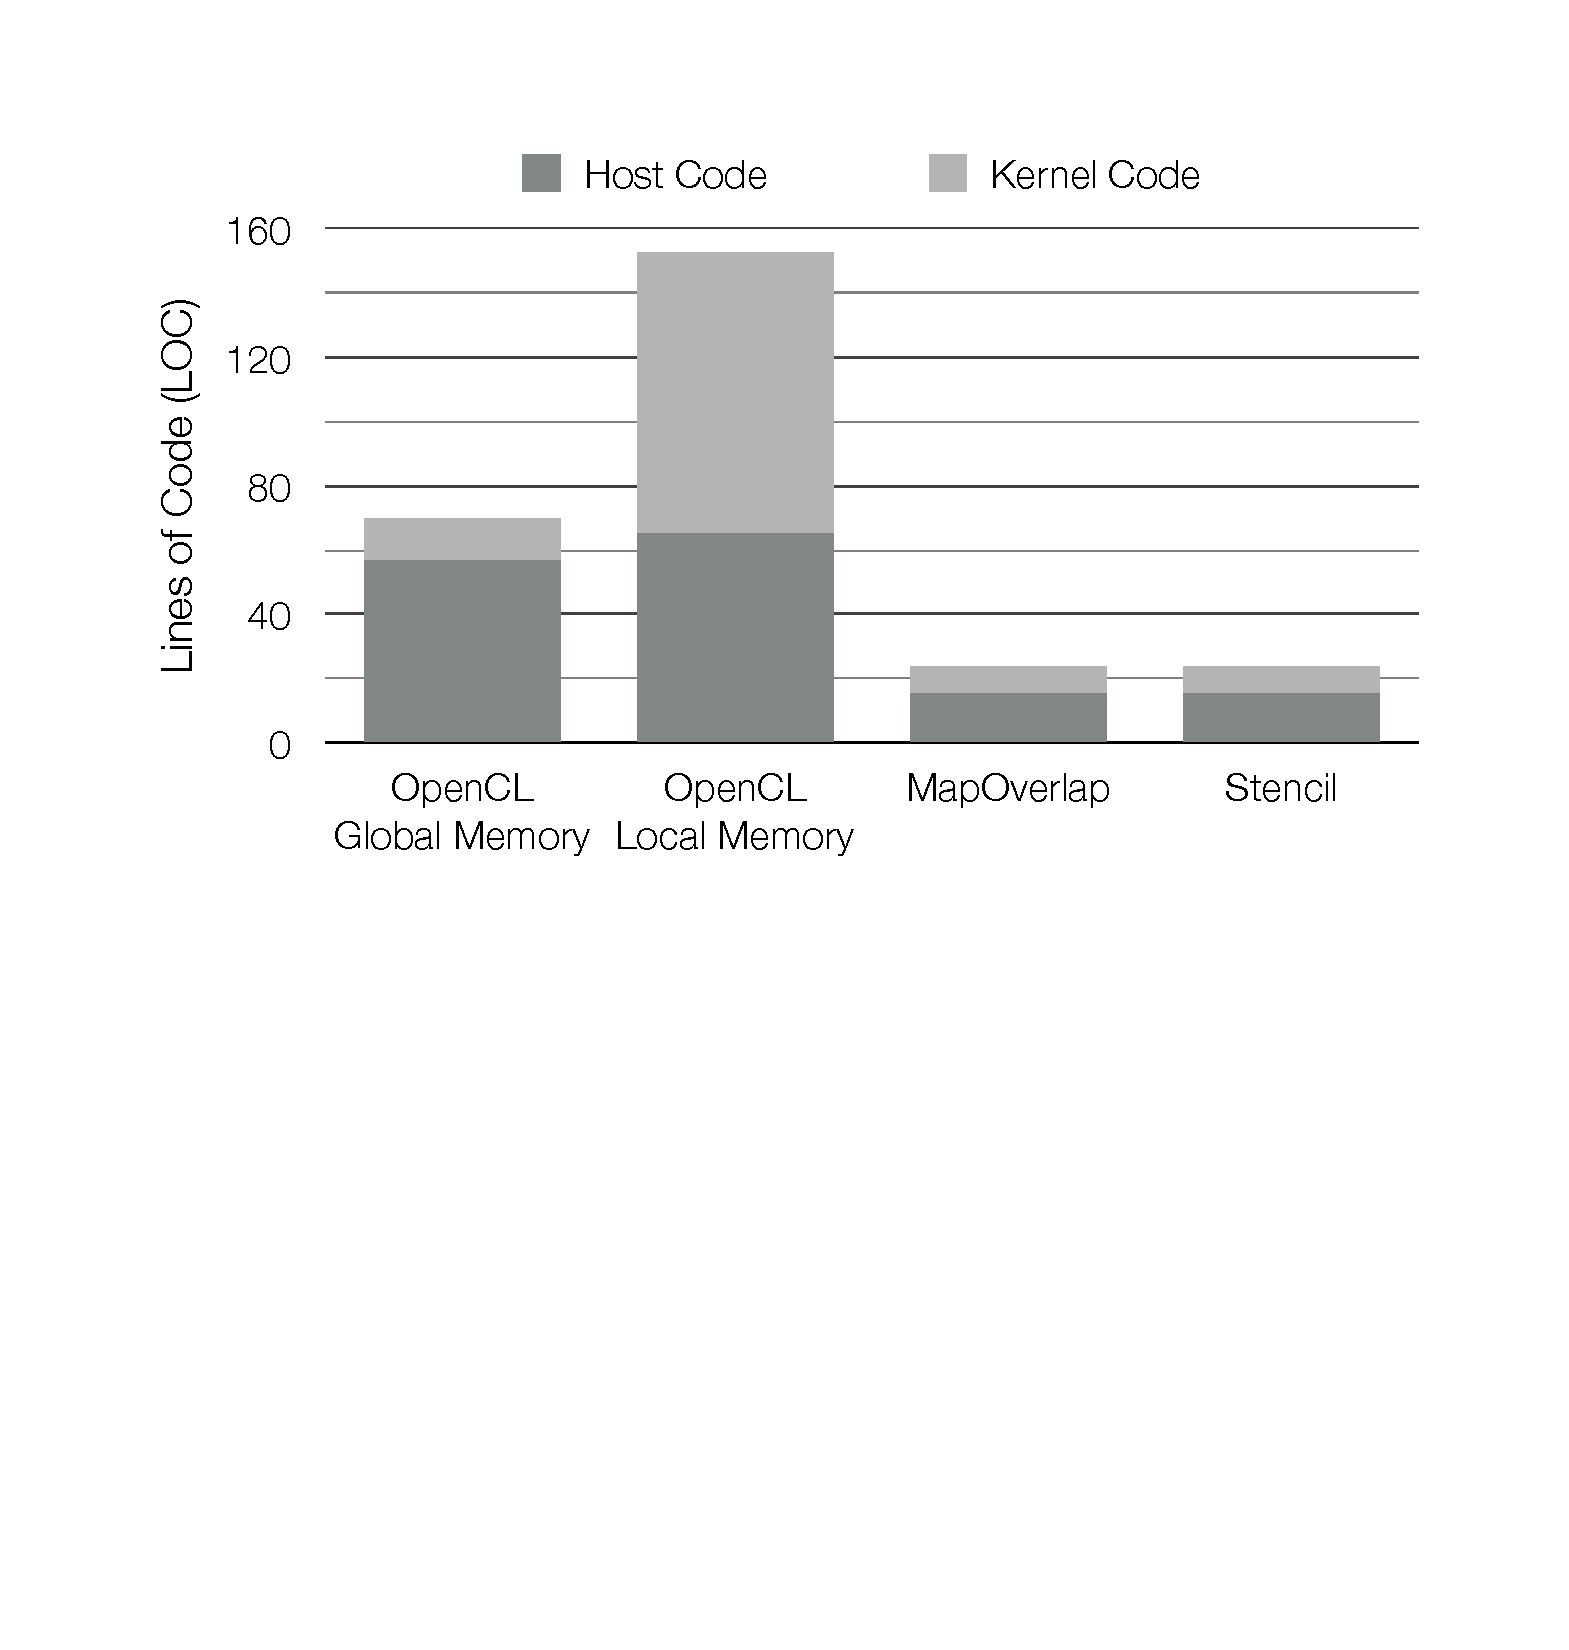
\includegraphics[width=\columnwidth]{HiStencils/LOC.pdf}
	\caption{Lines of code of the Gaussian blur using a na{\"i}ve OpenCL implementation with global memory, an optimized OpenCL version using local memory and \SkelCL's \code{MapOverlap} and \code{Stencil} implementations of the \stencil skeleton.}
	\label{fig:gaussLOCs}
\end{figure} 

\autoref{fig:gaussLOCs} shows the program sizes (in lines of code) for the four implementations. 
The application developer needs $57$ lines of OpenCL host code and 13 LOCs for performing a Gaussian blur with global memory. 
When using local memory, some more arguments are passed to the kernel, increasing the host-LOCs to $65$, while the LOCs for the kernel function, which copies all necessary elements for a work-group's calculation into local memory, requires $88$ LOCs with explicit out-of-bounds handling and complex index calculations.
\code{MapOverlap} and \code{Stencil} are similar to use and both require only $15$ LOCs host code and $9$ LOCs kernel code to perform a Gaussian blur. 
The support for multi-\GPU systems is implicitly given when using \SkelCL's skeletons, such that the kernel remains the same as for one-\GPU systems.
This is an important advantage of \SkelCL over the \OpenCL implementations of the Gaussian blur which are single-\GPU only, and they require additional LOCs when fitting to multi-\GPU environments.

The implementations using MapOverlap and Stencil are only $5-10\%$ slower than an optimized OpenCL implementation of the Gaussian blur while being much shorter than the OpenCL version.

\subsubsection*{Performance experiments}

\begin{figure}[tbp]
	\centering
	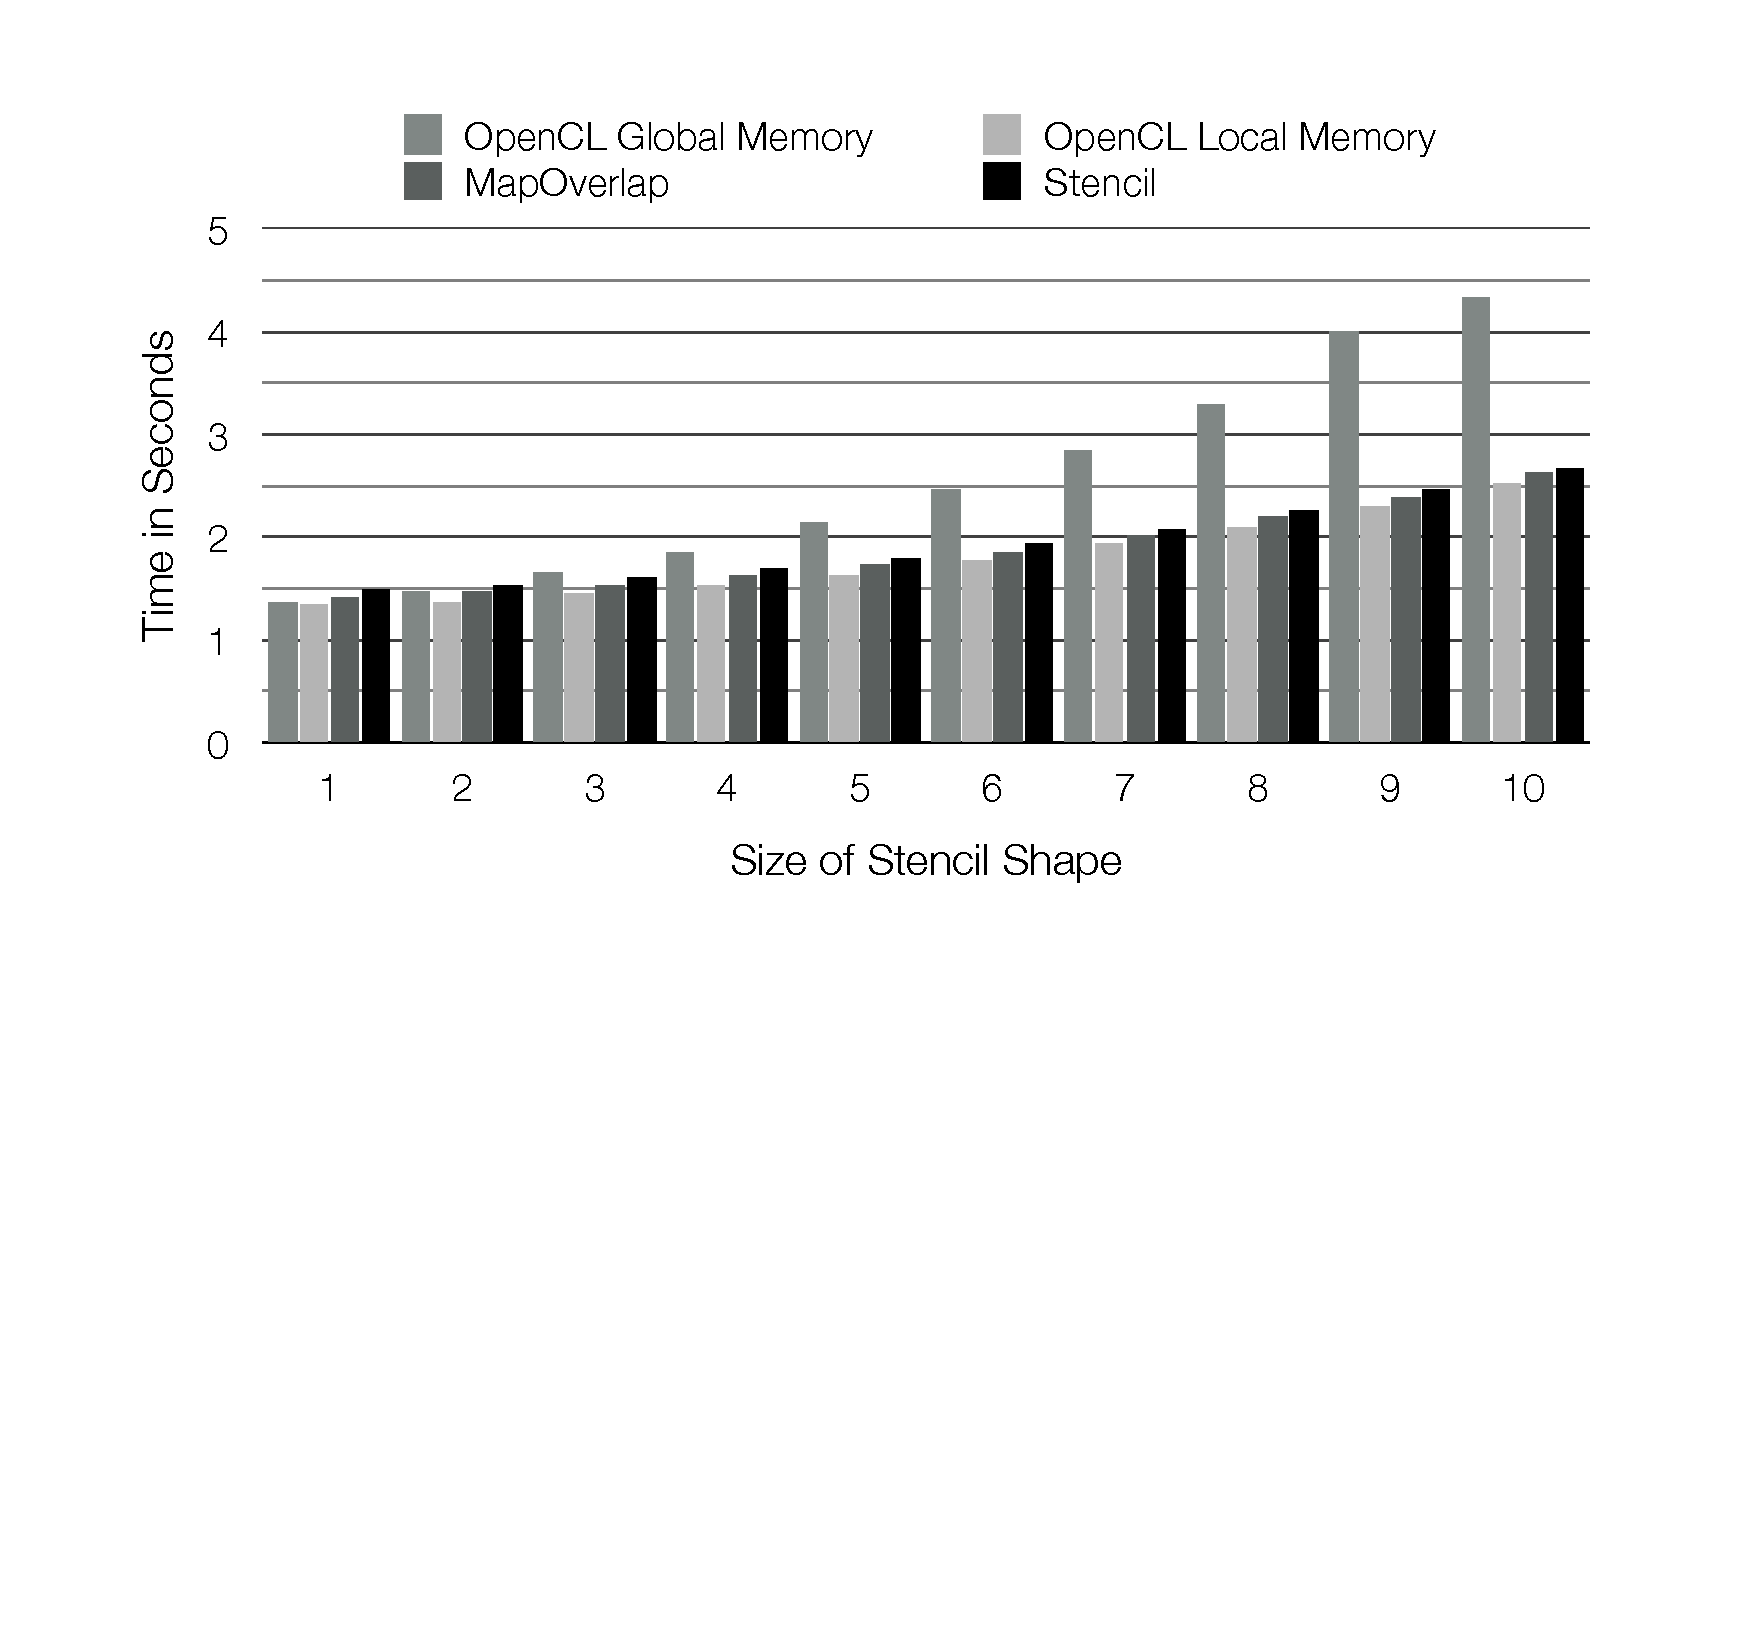
\includegraphics[width=\columnwidth]{HiStencils/GaussOpenCL.pdf}
	\caption{Runtime of the Gaussian blur using a na{\"i}ve OpenCL implementation with global memory, an OpenCL version using local memory and SkelCL's MapOverlap and Stencil skeletons.}
	\label{fig:gaussAbs}
\end{figure} 

\autoref{fig:gaussAbs} shows the total runtime of the Gaussian blur using:
1) a na{\"i}ve OpenCL implementation using global memory,
2) an optimized OpenCL version using local memory, and
3) the \code{MapOverlap} implementation, and
4) the \code{Stencil} implementation of the \stencil skeletons for different sizes of stencil shape, correspondingly.
We observe that on larger stencil shape sizes, \code{MapOverlap} and \code{Stencil} outperform the na{\"i}ve OpenCL implementation by $65\%$ and $62\%$, respectively.
The optimized OpenCL version, which copies all necessary elements into local memory prior to calculation, is $5\%$ faster than \code{MapOverlap} and $10\%$ faster than \code{Stencil} for small stencil shapes.
When increasing the stencil shape size, this disadvantage is reduced to $3\%$ for \code{MapOverlap} and $5\%$ for \code{Stencil} with stencil shape's extent of $10$ in each direction.

The \code{Stencil} implementation is slower for small stencil shapes than the \code{MapOverlap} implementation, up to $32\%$ slower for an stencil shape size of $1$.
This is due to the increased branching required in the \code{Stencil} implementation, as discussed in more detail in \autoref{sec:skelcl:stencil}.
However, this disadvantage is reduced to $4.2\%$ for an stencil shape size of $5$ and becoming negligible for bigger stencil shape sizes.
% Due to the increased branching in Stencil's kernel function, one might expect a worse runtime for the Stencil skeleton. 
As the ratio of copying into local memory decreases in comparison to the number of calculations when enlarging the stencil shape's extents, the \code{Stencil} implementation kernel function's runtime converges to the \code{MapOverlap} implementation's.
The \code{Stencil} implementation's disadvantage is also due to its ability to manage multiple stencil shapes and explicitly support the use of iterations.
While both features are not used in this use case, they incur some overhead for the implementation as compared to the \code{MapOverlap} implementation for simple stencil computations.


\autoref{fig:GaussMult} shows the speedup achieved on the Gaussian blur using the \code{Stencil} implementation on up to four devices.
The higher the computational complexity for increasing size of stencil shape, the better the overhead is hidden, leading to a maximum speedup of $1.90$ for two devices, $2.66$ for three devices, and $3.34$ for four devices.
\begin{figure}
	\centering
	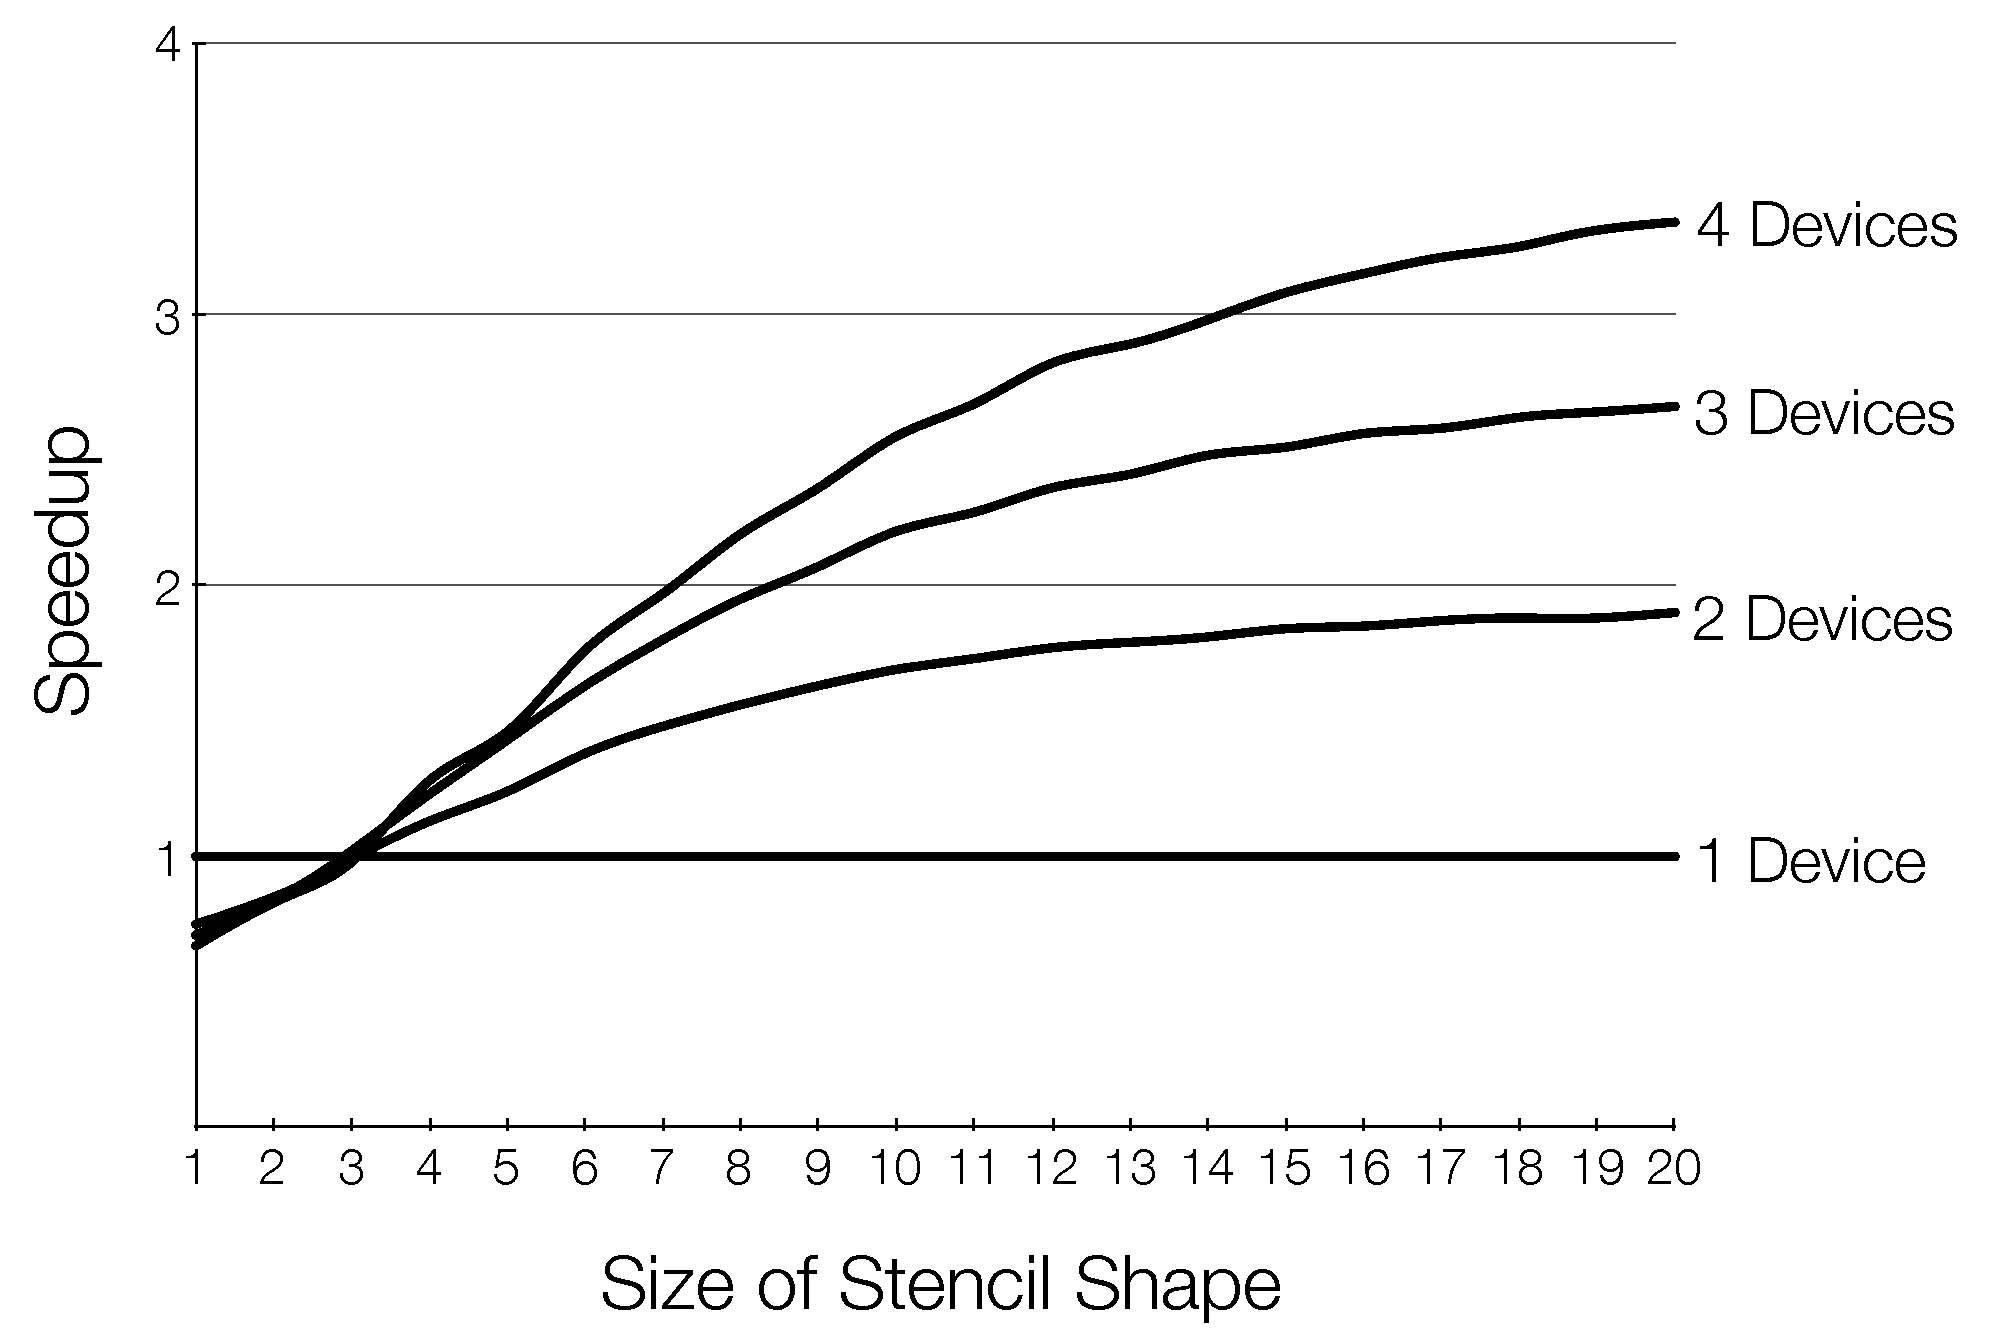
\includegraphics[width=.85\columnwidth]{HiStencils/SpeedupGauss.pdf}
	\caption{Speedup on up to four \GPUs.}
	\label{fig:GaussMult}
\end{figure} 










\subsection{Sobel edge detection}
\label{sec:sobel}
The Sobel edge detection produces an output image in which the detected edges in the input image are marked in white and plain areas are shown in black.
The effect is shown in \autoref{fig:sobel:lena}, where the original image is shown on the left and the output of Sobel edge detection applied to it on the right.

\begin{figure}[tb]
  \centering
  \begin{subfigure}[t]{.45\textwidth}
    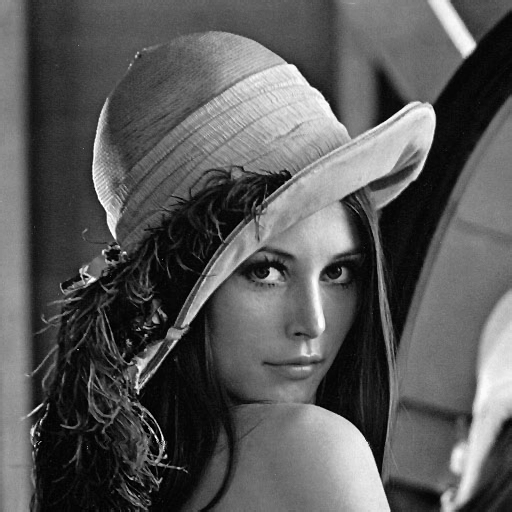
\includegraphics[width=\textwidth]{Paraphrase/lena.png}
    \caption{Original image.}
    \label{fig:lena:orig}
  \end{subfigure}
  \hfill
  \begin{subfigure}[t]{.45\textwidth}
    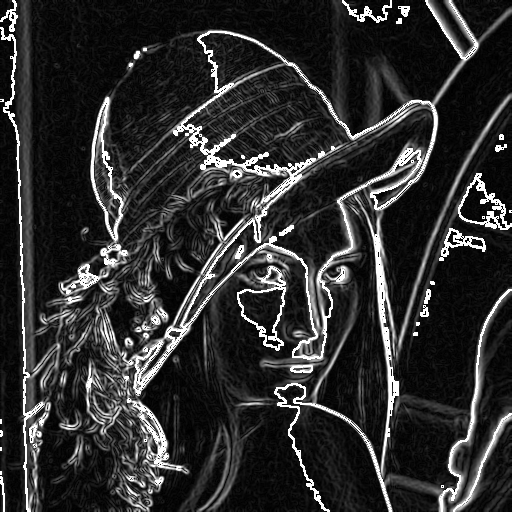
\includegraphics[width=\textwidth]{Paraphrase/sobel_filtered-lena.png}
    \caption{Image after Sobel edge detection.}
    \label{fig:lena:sobel}
  \end{subfigure}
  \caption{The famous Lena image~\cite{Lena} often used as an example in image processing before (left) and after (right) applying Sobel edge detection.}
  \label{fig:sobel:lena}
\end{figure}

\begin{lstlisting}[%
caption={Sequential implementation of the Sobel edge detection.},%
float=tb,
label={lst:sobel:seq}]
for (i = 0; i < width; ++i)
  for (j = 0; j < height; ++j)
    h = -1*img[i-1][j-1] +1*img[i+1][j-1]
        -2*img[i-1][j  ] +2*img[i+1][j  ]
        -1*img[i-1][j+1] +1*img[i+1][j+1];
    v = ...;
    out_img[i][j] = sqrt(h*h + v*v);
\end{lstlisting}
\bigskip

\autoref{lst:sobel:seq} shows the algorithm of the Sobel edge detection in pseudo-code, with omitted boundary checks for brevity.
In this sequential version, for computing an output value \code{out\_img[i][j]} the input value \code{img[i][j]} and the direct neighboring elements are needed.
Therefore, the \stencil skeleton is a perfect fit for implementing the Sobel edge detection.

\subsubsection*{\SkelCL Implementation}
\autoref{eq:sobel} shows the implementation of the Sobel edge detection in \SkelCL.
\begin{align}
  \label{eq:sobel}
  sobel\ M& = stencil\ f\ 1\ \overline{0}\ M \qquad\text{where:}\\
  f\ &\left[\begin{array}{lll}%
      \hspace{-.5em} M_{i-1,j-1}& \hspace{-.5em} M_{i-1,j} & \hspace{-.5em}M_{i-1,j+1}\vspace{-.25em}\\%
      \hspace{-.5em} M_{i,j-1}& \hspace{-.5em} M_{i,j} & \hspace{-.5em}M_{i,j+1}\vspace{-.25em}\\%
      \hspace{-.5em} M_{i+1,j-1}& \hspace{-.5em} M_{i+1,j} & \hspace{-.5em}M_{i+1,j+1}
    \end{array}\right] = \displaystyle\sqrt{ h^2 + v^2 }\nonumber\\
  h & = \sum_{k=0}^2 \sum_{l=0}^2 Gx_{k, l}\cdot M_{i+k-1,j+k-1}\nonumber\\
  v & = \sum_{k=0}^2 \sum_{l=0}^2 Gy_{k, l}\cdot M_{i+k-1,j+k-1}\nonumber\\
  Gx& = \left[\begin{array}{ccc}%
      -1&0&+1\\
      -2&0&+2\\
      -1&0&+1
    \end{array}\right]
  Gy = \left[\begin{array}{ccc}%
      -1&-2&-1\\
      0&0&0\\
      +1&+2&+1
    \end{array}\right] \nonumber\\
  \text{and } \overline{0} \text{ is th}&\text{e constant function always returning 0.}\nonumber
\end{align}
The formula resembles the sequential implementation shown in \autoref{lst:sobel:seq} where the final result is computed as the square root of the sum of two squared terms $h$ and $v$.
These are computed as weighted sums of the neighboring values $M_{i,j}$.
The weights are given by the two matrices $Gx$ and $Gy$.

\autoref{lst:sobel:skelcl} shows the \SkelCL implementation using the \code{MapOverlap} implementation of the \stencil skeleton.
%
\begin{lstlisting}[%
caption={\SkelCL implementation of the Sobel edge detection.},%
numbers=left,
float=tb,
label={lst:sobel:skelcl}]
Matrix<char> sobelEdge(const Matrix<char>& image) {
  auto sobel = mapOverlap(
    [](Neighborhood<char>& in) {
      short h = -1*in[{-1,-1}] +1*in[{+1,-1}]
                -2*in[{-1, 0}] +2*in[{+1, 0}]
                -1*in[{-1,+1}] +1*in[{+1,+1}];
      short v = ...;
      return sqrt(h*h + v*v); },
    1, BorderHandling::NEUTRAL(0));
  return soble(img); }
\end{lstlisting}
%
The implementation is straightforward and very similar to the formula in \autoref{eq:sobel} and the sequential version in \autoref{lst:sobel:seq}.

\subsubsection*{Programming effort}

\begin{lstlisting}[%
caption={Additional boundary checks and index calculations for Sobel algorithm, necessary in the standard OpenCL implementation.},%
float=tb,
numbers=left,
label={lst:sobel:opencl}]
kernel void sobel_kernel( global const uchar* img,
                          global       uchar* out_img) {
 uint i = get_global_id(0);   uint j = get_global_id(1);
 uint w = get_global_size(0); uint h = get_global_size(1);
 // perform boundary checks
 if(i >= 1 && i < (w-1) && j >= 1 && j < (h-1)) {
  char ul = img[((j-1)*w)+(i-1)];
  char um = img[((j-1)*w)+(i+0)];
  char ur = img[((j-1)*w)+(i+1)];
  // ... 5 more
  char lr = img[((j+1)*w)+(i+1)];

  out_img[j * w + i] = computeSobel(ul, um, ur, ..., lr); }}
\end{lstlisting}

\autoref{lst:sobel:opencl} shows a part of the rather simple \OpenCL implementation for Sobel edge detection provided by AMD as an example for their software development kit~\cite{AMDSDK}.
The actual computation is performed inside the \texttt{computeSobel} function, which is omitted in the listing, since it is quite similar to the sequential version in \autoref{lst:sobel:seq}.
The listing shows that extra low-level code is necessary to deal with technical details, like boundary checks and index calculations, which are arguably complex and error-prone.

We also compare against a more optimized \OpenCL implementation by Nvidia which makes use of the fast local \GPU memory.

The \SkelCL implementation is significantly shorter than the cumbersome \OpenCL implementations.
The \SkelCL program only comprises the few lines of code shown in \autoref{lst:sobel:skelcl}.
The AMD implementations requires 37 lines of code for its kernel implementation and the more optimized Nvidia implementation requires even 208 lines of code.
Both versions require additional lines of code for the host program which manages the execution of the \OpenCL kernel.
No index calculations or boundary checks are necessary in the \SkelCL version whereas they are crucial for a correct implementation in \OpenCL.

\subsubsection*{Performance experiments}

\begin{figure}[tbp]
  \vspace{.5em}
  \centering
  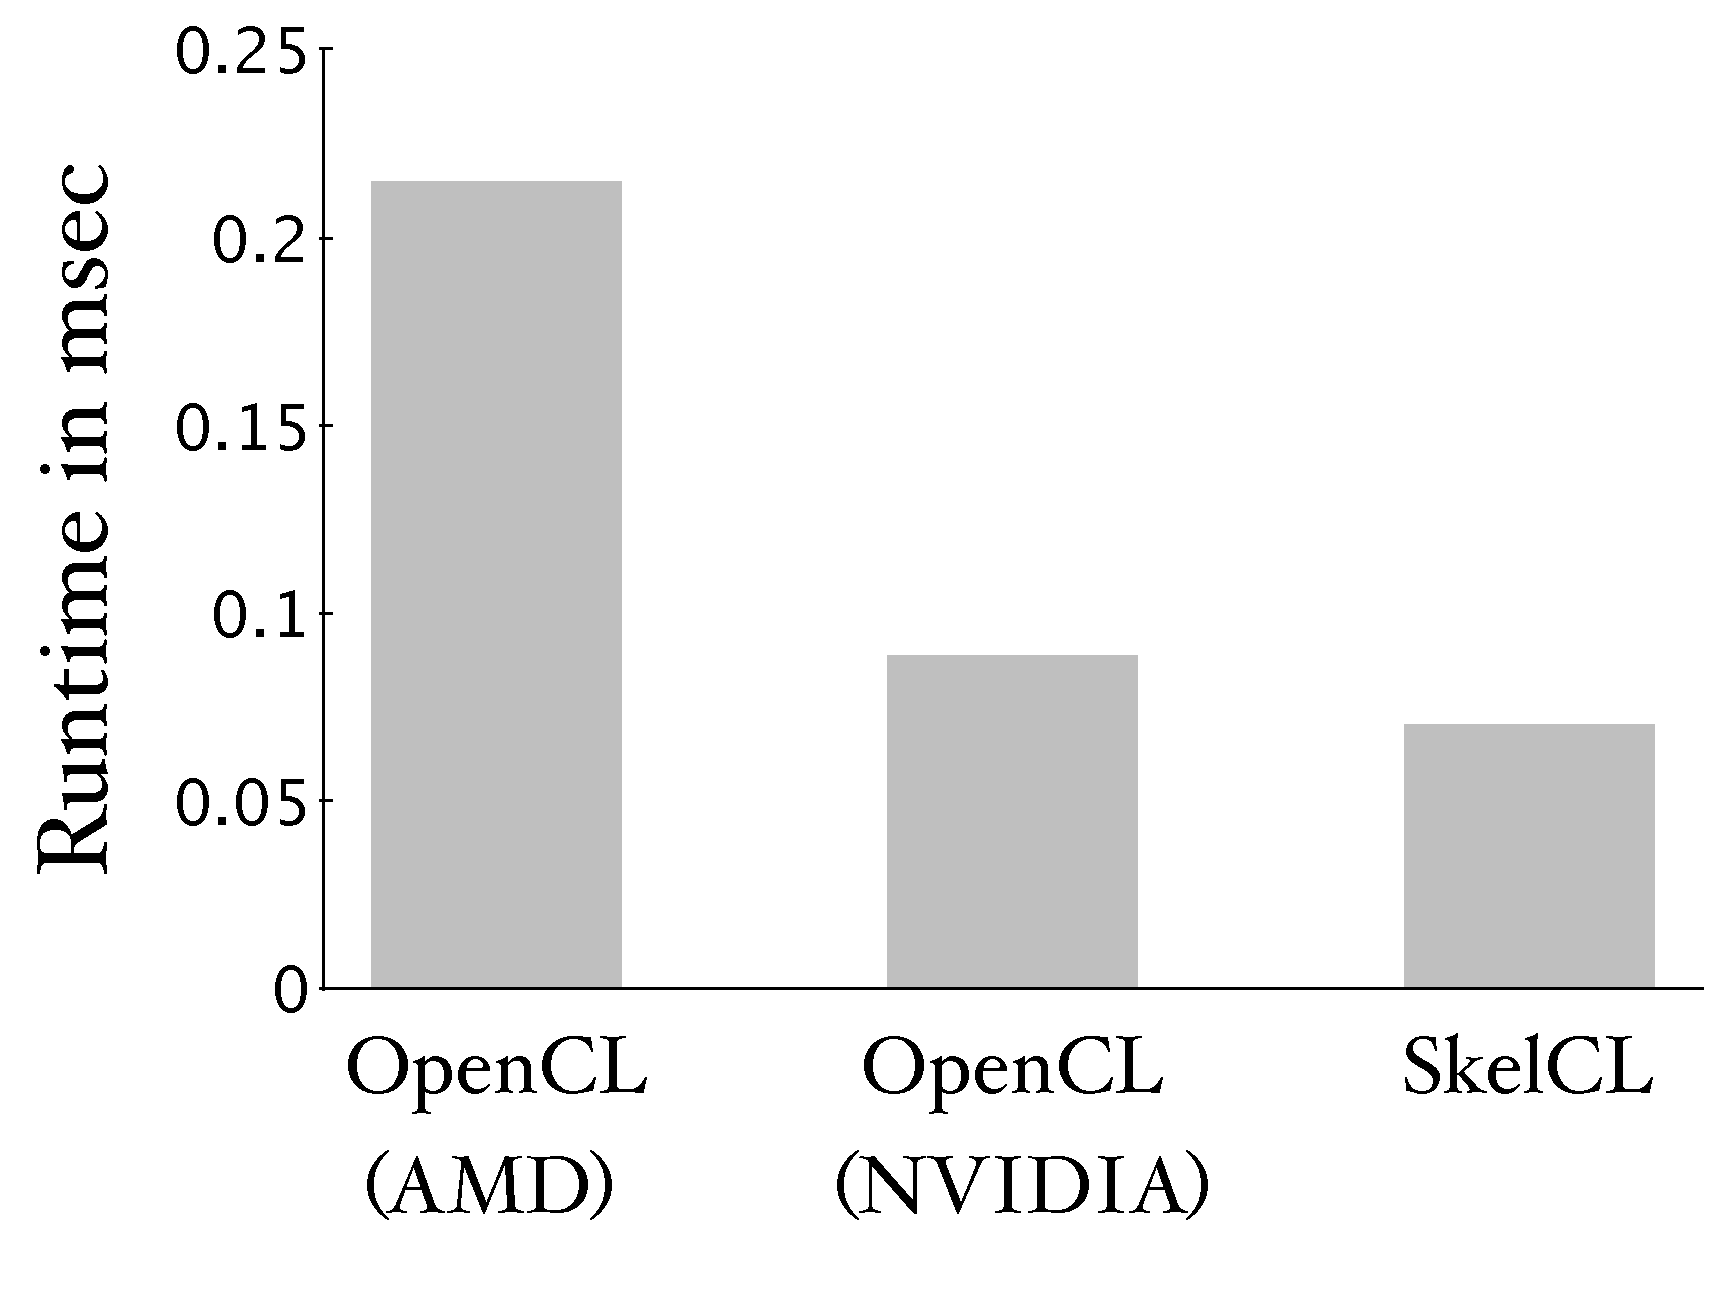
\includegraphics[height=4.5cm]{PaCT/lena.pdf}
  \caption{Performance results for Sobel edge detection}
  \label{fig:sobel:measurements}
\end{figure}
\autoref{fig:sobel:measurements} shows the runtime of two \OpenCL versions (from the AMD and Nvidia SDKs) vs. the \SkelCL version with the \stencil skeleton presented in \autoref{lst:sobel:skelcl}.
Here only the kernel runtimes are shown, as the data transfer times are equal for all versions.
We used the popular Lena image~\cite{Lena} with a size of $512\times 512$ pixel.
The AMD version is clearly slower then the two other implementations, because it does not use the fast local memory which the Nvidia implementation and the \code{MapOverlap} implementation of the \stencil skeleton of \SkelCL do.
\SkelCL completely hides the memory management details inside its implementation from the application developer.
The Nvidia and \SkelCL implementations perform similar.
In this particular example, \SkelCL even slightly outperforms the implementation by Nvidia.










\subsection{Canny Edge Detection}
The Canny edge detection algorithm is a more complex algorithm to detect edges in images than the Sobel edge detection presented in the previous section.
For the sake of simplicity we consider a slightly simplified version, which applies the following stencil operations in a sequence:
1), a noise reduction operation is applied, \eg, a Gaussian blur;
2), an edge detection operator like the Sobel edge detection is applied;
3), the so-called non-maximum suppression is performed, where all pixels in the image are colored black except pixels being a local maximum;
4), a threshold operation is applied to produce the final result.
A more complex version of the algorithm performs the edge tracking by hysteresis, as an additional step.
This results in detecting some weaker edges, but even without this additional step the algorithm usually achieves good results.


\subsubsection*{\SkelCL Implementation}
In \SkelCL, each single step of the Canny algorithm can be expressed using the \stencil skeleton.
The last step, the threshold operation, does not need access to neighboring elements, as the user threshold function only checks the value of the current pixel.
Therefore, this step can be expressed using \SkelCL's simpler \map skeleton.
In the \SkelCL library the \code{Stencil} skeleton's implementation automatically uses the simpler \map skeleton's implementation when the user specifies a stencil shape which extents are $0$ in all directions.

\begin{lstlisting}[%
  caption={Structure of the Canny algorithm as implemented with a sequence of skeletons.},%
  float=tbp,%
  label={lst:skelcl:canny}]
Matrix<char> sobelEdge(const Matrix<char>& image) {
  auto gauss     = stencil(...);$\label{lst:skelcl:canny:step1}$
  auto sobel     = stencil(...);
  auto nms       = stencil(...);
  auto threshold = stencil(...);$\label{lst:skelcl:canny:stepN}$
  StencilSequence<Pixel(Pixel)>
      canny(gauss, sobel, nms, threshold);$\label{lst:skelcl:canny:combine}$
  return canny(image); }$\label{lst:skelcl:canny:call}$
\end{lstlisting}

To implement the Canny algorithm in SkelCL, the single steps can be combined as shown in \autoref{lst:skelcl:canny}.
The individual steps are defined in lines~\ref{lst:skelcl:canny:step1}--\ref{lst:skelcl:canny:stepN} and then combined to a sequence of stencils in line~\ref{lst:skelcl:canny:combine}.
During execution (line~\ref{lst:skelcl:canny:call}), the stencil operations are performed in the order which is specified when creating the \emph{StencilSequence} object.

\subsubsection*{Programming effort}
\todo{...}

\subsubsection*{Performance experiments}

\begin{figure}[tbp]
	\centering
	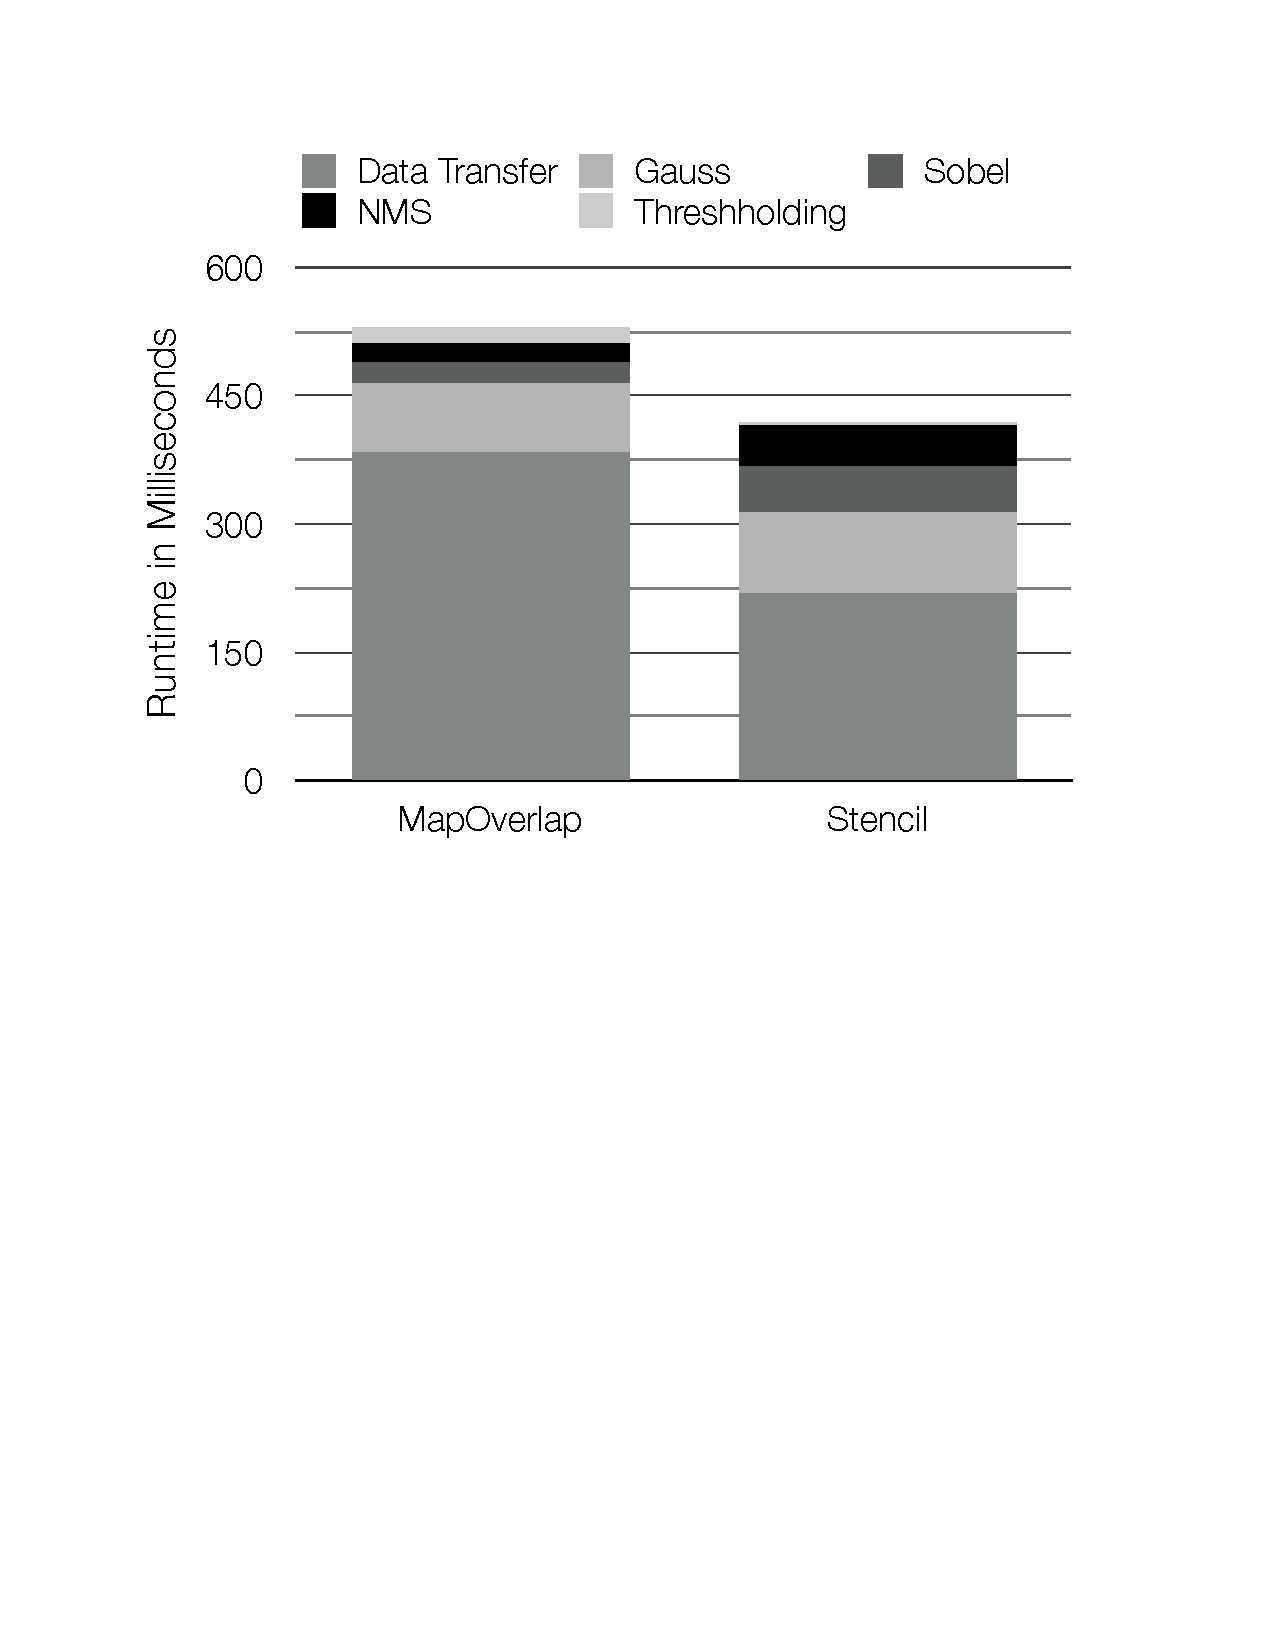
\includegraphics[width=.9\columnwidth]{HiStencils/Canny.pdf}
	\caption{Runtime of the Canny edge detection algorithm comparing the \code{MapOverlap} and \code{Stencil} skeleton implementations.}
	\label{fig:canny}
\end{figure} 

\autoref{fig:canny} shows the absolute runtime of the Canny algorithm. 
As the \code{MapOverlap} implementation appends padding elements to the matrix, the matrix has to be downloaded, resized and uploaded again to the \GPU between each step of the sequence.
This additional work to an increased time for data transfers. 
The Gaussian blur with a stencil shape extent of $2$, as well as the Sobel edge detection and the non-maximum suppression with a stencil shape of $1$, are $2.1$ to $2.2$ times faster when using \code{MapOverlap}. 
However, the threshold operation, which is expressed as the \map skeleton in the Stencil sequence, is $6.8$ times faster than \code{MapOverlap}'s threshold operation.
Overall, when performing sequences of stencil operations, the \code{Stencil} implementation reduces the number of copy operations and, therefore, leads to a better overall performance.
When performing the Canny algorithm, the \code{Stencil} implementation outperforms the \code{MapOverlap} implementation by $21\%$.



\section{Medical Imaging}
\label{section:medical-imaging}
At the beginning of \autoref{chapter:skelcl} we used the LM OSEM medical imaging application as our motivational example and application study to identify requirements for a high-level programming model.
In this section we will now study how we can express the LM OSEM application using algorithmic skeletons and how the parallel container data types and \SkelCL's redistribution feature simplify the programming of multi-GPU systems.
We will start by briefly reintroducing the application and its sequential implementation before moving to the parallel implementation using first traditional \OpenCL and then \SkelCL for comparison.
A particular focus of this section will be on multi-GPU systems and how \SkelCL radically simplifies their programming.

\subsubsection*{The LM OSEM Algorithm}
\emph{List-Mode Ordered Subset Expectation Maximization} (LM OSEM)~\cite{ReaderErFlOt1998, SchellmannGoMeKoScWuBu2009} is a time-intensive, production-quality algorithm for medical image reconstruction.
LM OSEM takes a set of events from a PET scanner and splits them into $s$ equally sized subsets.
Then, for each subset $S_l, l \in {0, \ldots, s-1}$, the following computation is performed:
\begin{equation}
 f_{l+1}=f_{l}c_{l};\quad
 c_{l}=\dfrac{1}{A_N^T \textbf{1}}
\sum_{i \in S_{l}} (A_i)^T \dfrac{1}{A_{i} f_{l}}.
\label{eq:lm_osem2}
\end{equation}
Here $f$ is the 3D reconstruction image which is refined over time.
$A$ is a matrix where element $a_{ik}$ of row $A_i$ represents the length of intersection of the line between two PET detectors for a measured event $i$ with voxel $k$ of the reconstruction image.
The factor in front of the sum can be precomputed and is, therefore, omitted from here on.

\paragraph{Sequential implementation}
\autoref{lst:lmosem:seq_code:2} shows the sequential code for LM OSEM as already presented in \autoref{section:opencl-example}.
%
\begin{figure}
\begin{lstlisting}[
  caption={[Sequential code for LM OSEM.]Sequential code for LM OSEM comprises one outer loop with two nested inner loops.},
  label={lst:lmosem:seq_code:2}]
for (int l = 0; l < subsets; l++) {$\label{lst:lmosem:seq_core:2:loop}$
  // read subset

  // step 1: compute error image $c_l$
  for (int i = 0; i < subset_size; i++) { $\label{lst:lmosem:seq_code:2:step1:begin}$
    // compute $A_i$
    // compute local error
    // add local error to $c_l$
  } $\label{lst:lmosem:seq_code:step1:end}$

  // step 2: update reconstruction image $f$
  for (int k = 0 ; k < image_size; k++) { $\label{lst:lmosem:seq_code:2:step2:begin}$
    if (c_l[k] > 0.0) { f[k] = f[k] * c_l[k]; }
  } $\label{lst:lmosem:seq_code:2:step2:end}$
}
\end{lstlisting}
\end{figure}
%
The sequential LM OSEM is an iterative algorithm refining the reconstruction image $f$ over time, at each iteration two major steps are performed:
\begin{itemize}
  \item[] \emph{Step 1:} the error image $c_l$ is computed by performing three sub-steps: 1) computation of the row $A_i$; 2) computing the local error for row $A_i$; 3) adding the local error to $c_l$;
  \item[] \emph{Step 2:} update the reconstruction image $f$ using the error image $c_l$ computed in Step 1.
\end{itemize}

\paragraph{Parallelization strategy}
For parallelization two possible decomposition strategies can be considered for the LM OSEM algorithm as initially suggested in~\cite{JonesJoKeNeReLeByBaMiCa2002}: Projection Space Decomposition (PSD) and Image Space Decomposition (ISD).

In PSD, the subsets $S_l$ are split into sub-subsets that are processed simultaneously while all processing units access a common reconstruction image $f$ and error image $c$.
Using this approach, we are able to parallelize \emph{Step~1} of the algorithm, but \emph{Step~2} is performed by a single processing unit.
On a multi-\GPU system, we have to copy the reconstruction image to all \GPUs before each iteration, and we have to merge all \GPUs' error images computed in \emph{Step~1} before proceeding with \emph{Step~2}.
While both steps are easy to implement, \emph{Step~2} does not efficiently use the available processing units.

In ISD, the reconstruction image $f$ is partitioned, such that each processing unit processes the whole subset $S_l$ with respect to a single part of the reconstruction image $f$.
Thus we are able to parallelize both steps of LM OSEM, but each processing unit still accesses the whole reconstruction image $f$ in order to compute the error value for each path before merging it with the error image $c$.
On a multi-\GPU system, the whole subset $S_l$ has to be copied to each \GPU in \emph{Step~1}.
ISD requires large amounts of memory (up to several GB in practically relevant cases) to save all paths computed in \emph{Step~1}.
Summarizing, it is hard to implement \emph{Step~1} on the \GPU, while \emph{Step~2} can be parallelized easily.

Therefore, we use a hybrid strategy for implementing LM OSEM:
\emph{Step~1} is parallelized using the PSD approach, while we use ISD for \emph{Step~2}.
This results in the sequence of five phases shown in \autoref{fig:lmosem:em_distribution2}:
\begin{enumerate}
\item \emph{Upload:} the subset ($S$) is divided into sub-subsets (one per \GPU).
      One sub-subset and the reconstruction image ($f$) are uploaded to each \GPU;
\item \emph{Step 1:} each \GPU computes the local error image ($c_l$) for its sub-subset;
\item \emph{Redistribution:} the local error images that are distributed on all \GPUs are downloaded and combined into a single error image on the host by performing element-wise addition.
      Afterwards, the combined error image and reconstruction image are partitioned, in order to switch the parallelization strategy from PSD to ISD.
      The corresponding parts of both images are distributed to the \GPUs again;
\item \emph{Step 2:} each \GPU updates its part of the reconstruction image;
\item \emph{Download:} finally, all parts of the reconstruction image are downloaded from the \GPUs to the host and merged into a single reconstruction image.
\end{enumerate}

\begin{figure}
  \centering
  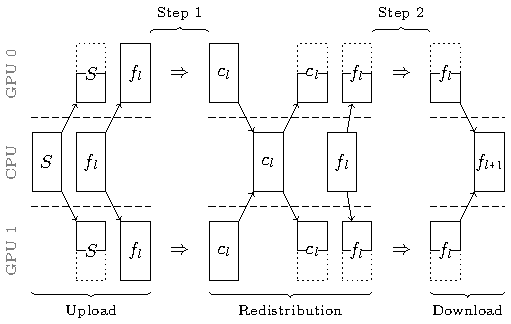
\includegraphics[width=0.6\textwidth]{ICCS/em_distribution}
  \caption{Parallelization schema of the LM OSEM algorithm.}
  \label{fig:lmosem:em_distribution2}
\end{figure}


\subsubsection*{\SkelCL Implementation}

The \SkelCL program in \autoref{lst:em_skelcl} reflects the described five phases in a concise, high-level manner, as shown by the corresponding comments.
The subset \code{s}, the error image \code{cl}, and the reconstruction image \code{f} are declared as \SkelCL vectors which enables an easy and automatic data transfer between \GPUs.
As data transfers are performed implicitly by \SkelCL, the upload phase is implemented by simply setting vector distributions (lines~\ref{lst:em:skelcl:upload:start}--\ref{lst:em:skelcl:upload:end}), while the download phase is performed implicitly when the \SkelCL containers are accessed or redistributed.
\begin{lstlisting}[%
  caption={SkelCL code of the LM OSEM algorithm},%
  numbers=left,%
float,%
label={lst:em_skelcl}]
auto computeCl = mapVector(
  [](Event e, const Vector<float>& f, Vector<float>& cl) {
    Path Ai = computeAi(e);$\label{lst:em:skelcl:computeAi}$
    float c = computeLocalError(f, Ai);
    addLocalErrorToCl(cl, c, Ai); });

auto updateF = zipVector(
  [](float f_i, float cl_i) {
    if (cl_i > 0.0) return f_i * cl_i; else return f_i; });

Vector<float> f   = readStartImage();
for (l = 0; l < subsets; l++) {
  Vector<Event> s = read_subset();
  Vector<float> cl(image_size);

  /* Upload */
  s.setDistribution(block);$\label{lst:em:skelcl:upload:start}$
  f.setDistribution(copy);
  cl.setDistribution(copy, add);$\label{lst:em:skelcl:upload:end}$

  /* Step 1: compute error image cl */
  computeCl(s, f, out(cl));$\label{lst:em:skelcl:execute}$

  /* Redistribution */
  f.setDistribution(block);$\label{lst:em:skelcl:redistribute:start}$
  cl.setDistribution(block);$\label{lst:em:skelcl:redistribute:end}$

  /* Step 2: update image estimate f */
  f = updateF(f, cl);

  /* Download (implicit) */}
\end{lstlisting}
The redistribution phase is implemented by changing the distributions of the corresponding \SkelCL containers (lines~\ref{lst:em:skelcl:redistribute:start} and~\ref{lst:em:skelcl:redistribute:end}).

The two computational steps are implemented using the \map and \zip skeleton from \SkelCL, correspondingly, as follows.

The first step -- the computation of the error image $c_l$ -- is implemented using the \map skeleton.
For each event \code{e} of the currently processed subset, the row $A_i$ is computed (line~\ref{lst:em:skelcl:computeAi}).
As $A_i$ is sparsely populated it is stored as a special data structure, called \code{Path}, to reduce its memory footprint.
Next, the local error is computed using $A_i$ together with the current reconstruction image $f$ which is passed to the \map skeleton as an additional argument.
Finally, the error image \code{cl} is updated with the local error.
The error image is also provided as an additional argument, but when executing the \map skeleton \code{cl} is wrapped using the \code{out} helper function (line~\ref{lst:em:skelcl:execute}).
This marks the additional argument as output parameter, \ie, the \SkelCL implementation is notified that this argument will be modified by the customizing function.
It is interesting to point out that the \map skeleton does not return a value, \ie, its return type is \code{void}.
The skeleton is only executed for its side effects on \code{cl}.

The second step -- the update of the reconstruction image $f$ -- is implemented using the \zip skeleton.
Here the customizing function operates on pairs of the voxels of the reconstruction and the error image, following the image space decomposition (ISD) strategy.
If the voxel of the error image is greater than zero, the voxel of the reconstruction image is updated with the product of the pair of voxels from the reconstruction and the error image.







\subsubsection*{Programming effort}
The lengthy and cumbersome \OpenCL implementation of the LM OSEM was already discussed in \autoref{chapter:skelcl}.
It is based on the work presented in~\cite{SchellmannGoMeKoScWuBu2009}.
\OpenCL requires a considerable amount of boilerplate code for running a kernel on multiple \GPUs, in particular for uploading and downloading data to and from the \GPUs.

The parallelization strategies are the same for both versions.
However, when using \SkelCL's vector data type, we avoid additional programming effort to implement data transfer between host and \GPU or between multiple \GPUs, and we obtain a multi-\GPU-ready implementation of LM OSEM for free.

\begin{figure}
  \centering
  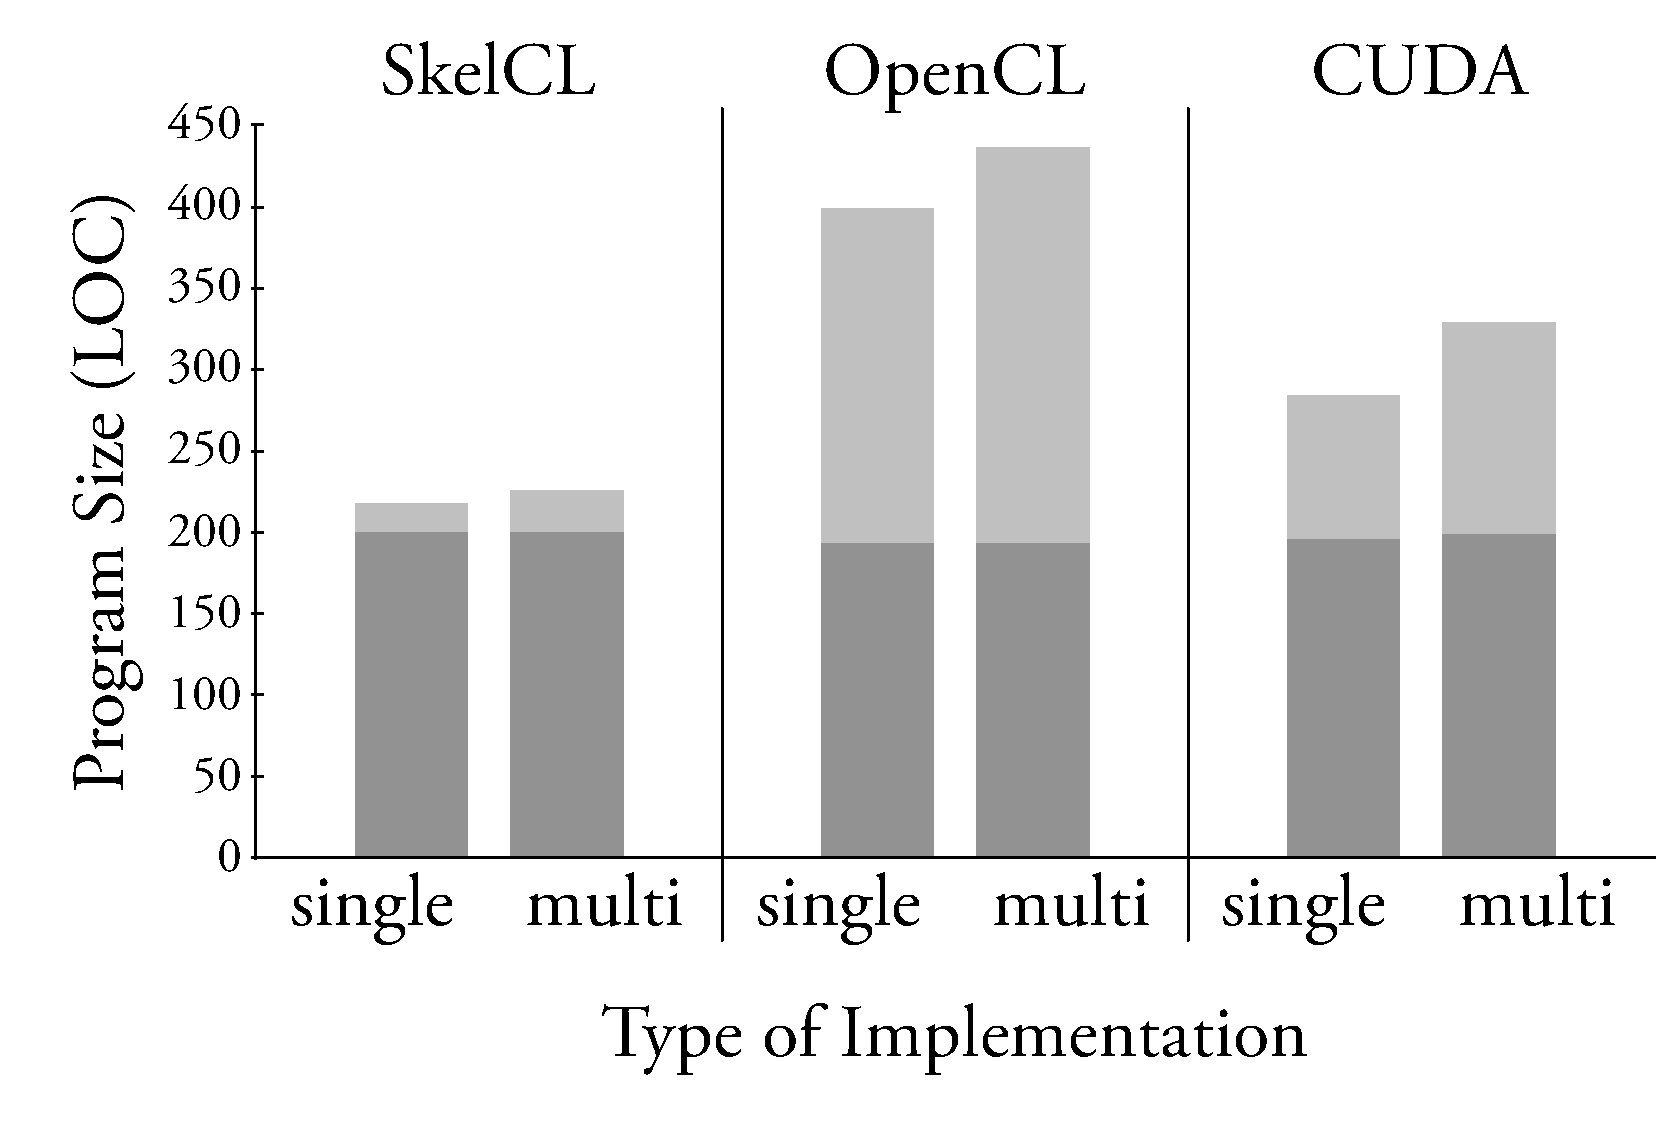
\includegraphics[width=.75\textwidth]{ASHES/loc}
  \caption[Lines of code of the LM OSEM implementations.]%
          {Lines of code for host (light gray) and \GPU (dark gray) of the LM OSEM implementations.}
  \label{fig:list-mode_OSEM:LOC}
\end{figure}

\autoref{fig:list-mode_OSEM:LOC} shows the lines of code required for both implementation.
The amount of lines required on the \GPU is similar.
This is not surprising, as these code describes the computation performed on the \GPU which is similar for both implementations.
The host code required for implementing the management of the \GPU execution differs significantly across implementations.
For a single \GPU, the \OpenCL-based implementation has the longest code (206 LOC), \ie, more than 11 times longer than the \SkelCL program which has 18 LOC.

Using multiple \GPUs in \OpenCL requires explicit code for additional data transfers between \GPUs.
This accounts for additional 37 LOC for the \OpenCL-based implementation.
In \SkelCL, only 8 additional LOC are necessary to describe the changes of data distribution.
These lines are easily recognizable in the \SkelCL program (lines~\ref{lst:em:skelcl:upload:start}--\ref{lst:em:skelcl:upload:end}, \ref{lst:em:skelcl:redistribute:start}--\ref{lst:em:skelcl:redistribute:end} in \autoref{lst:em_skelcl}, plus 3 lines during the initialization) and make this high-level code arguably better understandable and maintainable than the \OpenCL version.













\subsubsection*{Performance experiments}
We evaluated the runtimes of our two implementations of LM OSEM by reconstructing an image of $150\times 150\times 280$ voxels from a real-world PET data set with about $10^8$ events.
From this data set, about $10^2$ equally sized subsets are created.
In our experiments, we measured the average runtime of processing one subset.
To perform a full reconstruction producing a detailed reconstruction image, all subsets are processed multiple times, making LM OSEM a time-intensive application that runs several hours on a single-core \CPU.

\autoref{fig:list-mode_OSEM:runtime} shows the runtime of both implementations of LM OSEM using up to four \GPUs.
While the differences in the programming effort to implement the \SkelCL and \OpenCL versions are significant, the differences in runtime are quite small.
When running on a single \GPU, both implementations take the same time (3.66 seconds) to complete.
With two and four \GPUs, the \OpenCL implementation slightly outperforms the \SkelCL implementation, being 1.2\% and 4.7\% faster.
We presume that the increasing overhead of \SkelCL is caused by the more complex data distribution performed when using more \GPUs.
Comparing to the significant reduction in programming effort (50\%), the runtime overhead of less than 5\% is arguably a moderate one.
In conclusion, this example shows that \SkelCL is suitable for implementing a real-world application and provides performance close to a native \OpenCL implementation.

\begin{figure}
  \centering
  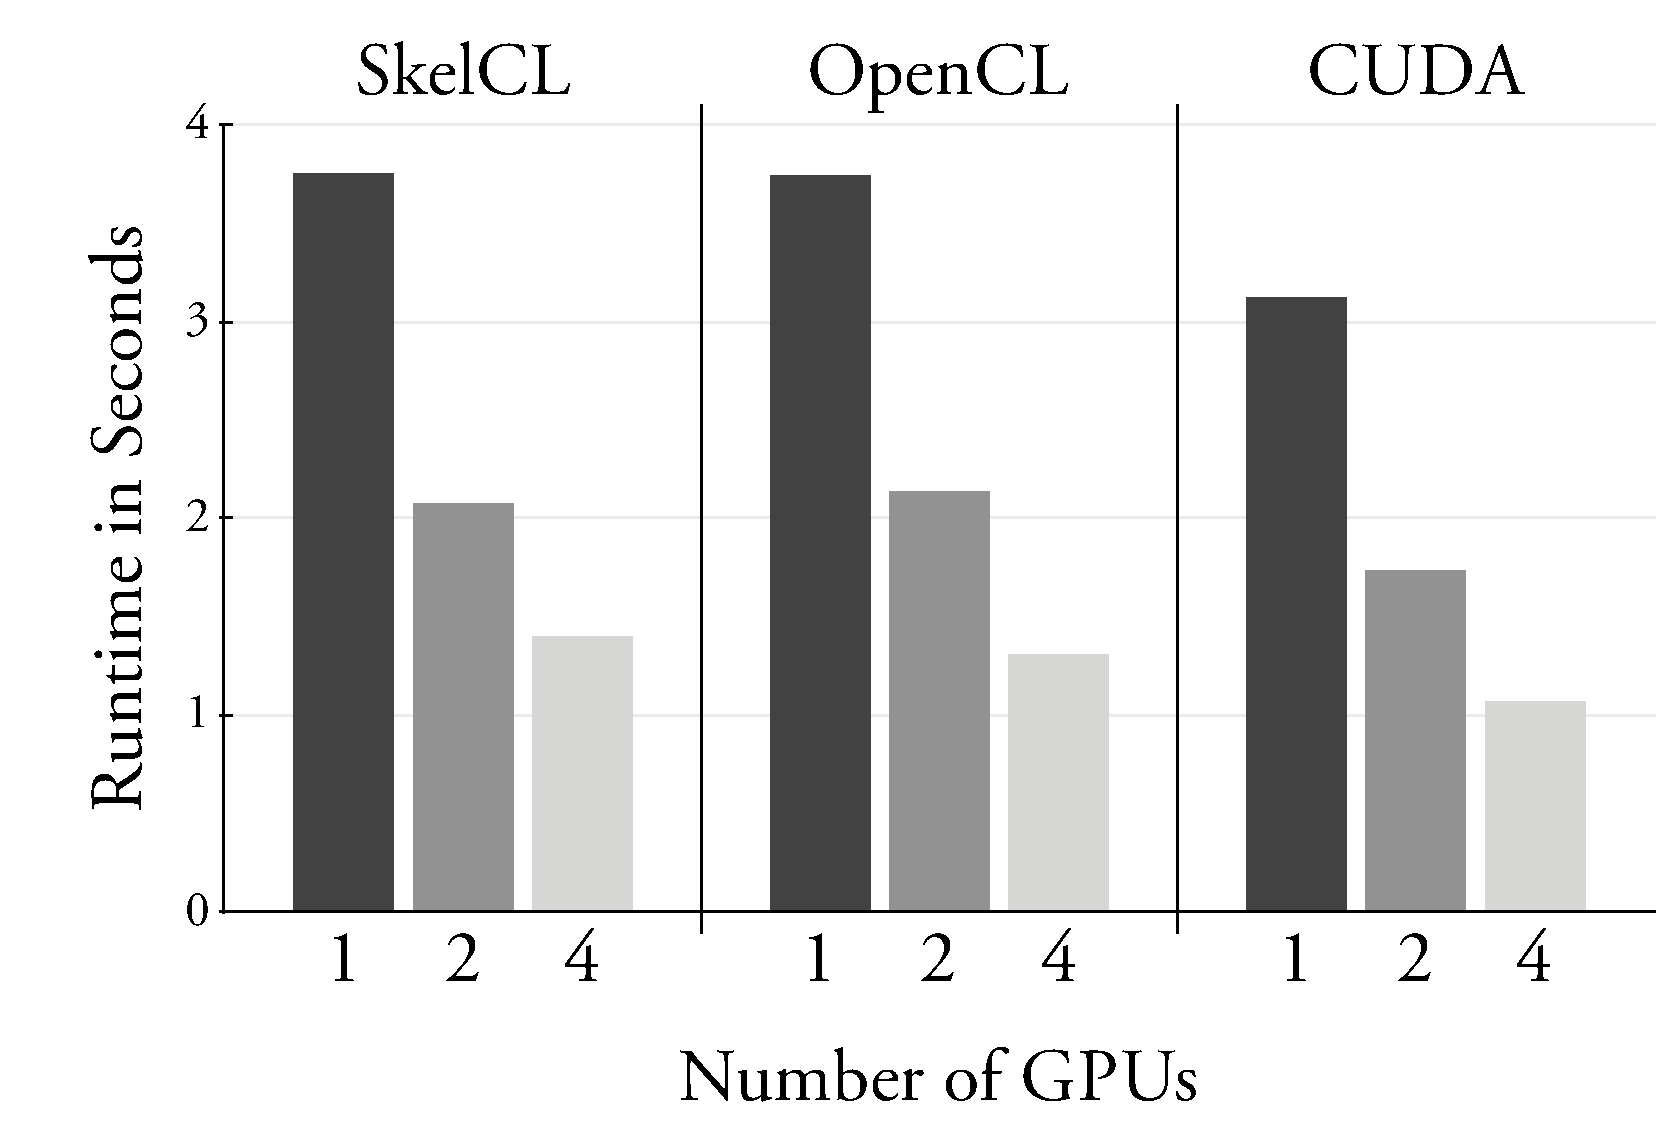
\includegraphics[width=.75\textwidth]{ASHES/lmosemIteration}
  \caption[Average runtime of one iteration of the LM OSEM algorithm.]%
          {Average runtime of one iteration of the LM OSEM algorithm using \SkelCL and \OpenCL.}
  \label{fig:list-mode_OSEM:runtime}
\end{figure}

%\begin{figure}
%  \centering
%  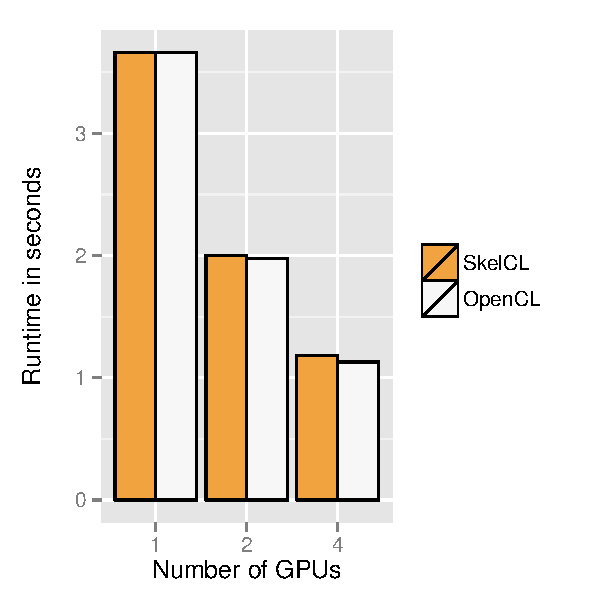
\includegraphics[width=.75\textwidth]{ICCS/skelcl-runtime.pdf}
%  \caption{Average runtime of one iteration of the LM OSEM algorithm using \SkelCL and \OpenCL.}
%  \label{fig:lmosem_runtime}
%\end{figure}



\section{Physics Simulation}
\label{sec:physicsSim}
\emph{Finite-Difference-Time-Domain (FDTD) Method for Random Lasing Simulations}
As our third application study we use a simulation from the field of optical physics, where the propagation of light through a medium is simulated.

In the simulation two fields, the electric field $\vec{E}$ and the magnetic field $\vec{H}$, are iteratively updated using stencils computations.
The Maxwell's equations are the basic equations describing electrodynamic processes in nature and are used here to describe the light propagating through a non-magnetic (\emph{dielectric}) medium.

\bigskip
\begin{minipage}{.44\linewidth}
\begin{equation} \vec{\nabla}\vec{E}\left(\vec{r}, t\right) = 0, \label{eq:div_e}\end{equation}
\end{minipage}
\hspace{.04\linewidth}
\begin{minipage}{.44\linewidth}
\begin{equation} \vec{\nabla}\vec{H}\left(\vec{r}, t\right) = 0, \label{eq:div_h}\end{equation}
\end{minipage}

\bigskip

\begin{minipage}{.44\linewidth}
\begin{equation} \frac{\partial\vec{H}\left(\vec{r}, t\right)}{\partial t} = -\frac{1}{\mu_0}\vec{\nabla} \times \vec{E}\left(\vec{r}, t\right), \label{eq:rot_h}\end{equation}
\end{minipage}
\hspace{.04\linewidth}
\begin{minipage}{.44\linewidth}
\begin{equation} \frac{\partial\vec{D}\left(\vec{r}, t\right)}{\partial t} = \frac{1}{\epsilon_0}\vec{\nabla} \times \vec{H}\left(\vec{r}, t\right), \label{eq:rot_d}\end{equation}
\end{minipage}
\bigskip

\newpage
\noindent
Eq. (\ref{eq:div_e})-(\ref{eq:rot_d}) show the Maxwell's equations consisting of four coupled partial differential equations (PDEs).
To couple the polarisation of a medium $\vec{P}$ to the electric field, Eq. (\ref{eq:flussdichte}) is introduced:

\begin{equation}
\vec{E}\left(\vec{r}, t\right) = \frac{\vec{D}\left(\vec{r}, t\right) - \vec{P}\left(\vec{r}, t, \vec{N}\right)}{\epsilon_0\epsilon_r\left(\vec{r}\right)}
\label{eq:flussdichte}
\end{equation}

\noindent
Here $\vec{N}$ is the induced energy distribution in the medium using the model proposed in~\cite{Jiang2000}.
The parameters $\mu_0$, $\epsilon_0$ and $\epsilon_r$ describe the permeability and permittivity of free space and the relative permittivity of the dielectric medium.

To solve this set of coupled PDEs, the Finite-Difference-Time-Domain Method (short FDTD)~\cite{Yee1966} can be used.
Here we use a form of FDTD where the electric and magnet field are discretized within a n-dimensional regular grid.
$\vec{E}$ and $\vec{H}$ are shifted against each other by a half grid-cell.
This allows the calculation of the new values by computing finite differences between two values of the grid.
Using the FDTD method, we implemented a simulation of the effect of random lasing on a nano-meter scale~\cite{Cao1999} for our evaluation.

Figure \ref{fig:fields} shows a visualization of the electric field (and the field intensity) after about  $1\,ps$ of simulation time equal to $60\,000$ iterations.
The shown field distribution can be found also in~\cite{Cao2000, Sebbah2002, Yamilov2005}.%, however the simulation parameters are different.

\begin{figure}[t]
	\begin{minipage}[b]{.48\textwidth}
    \centering
	  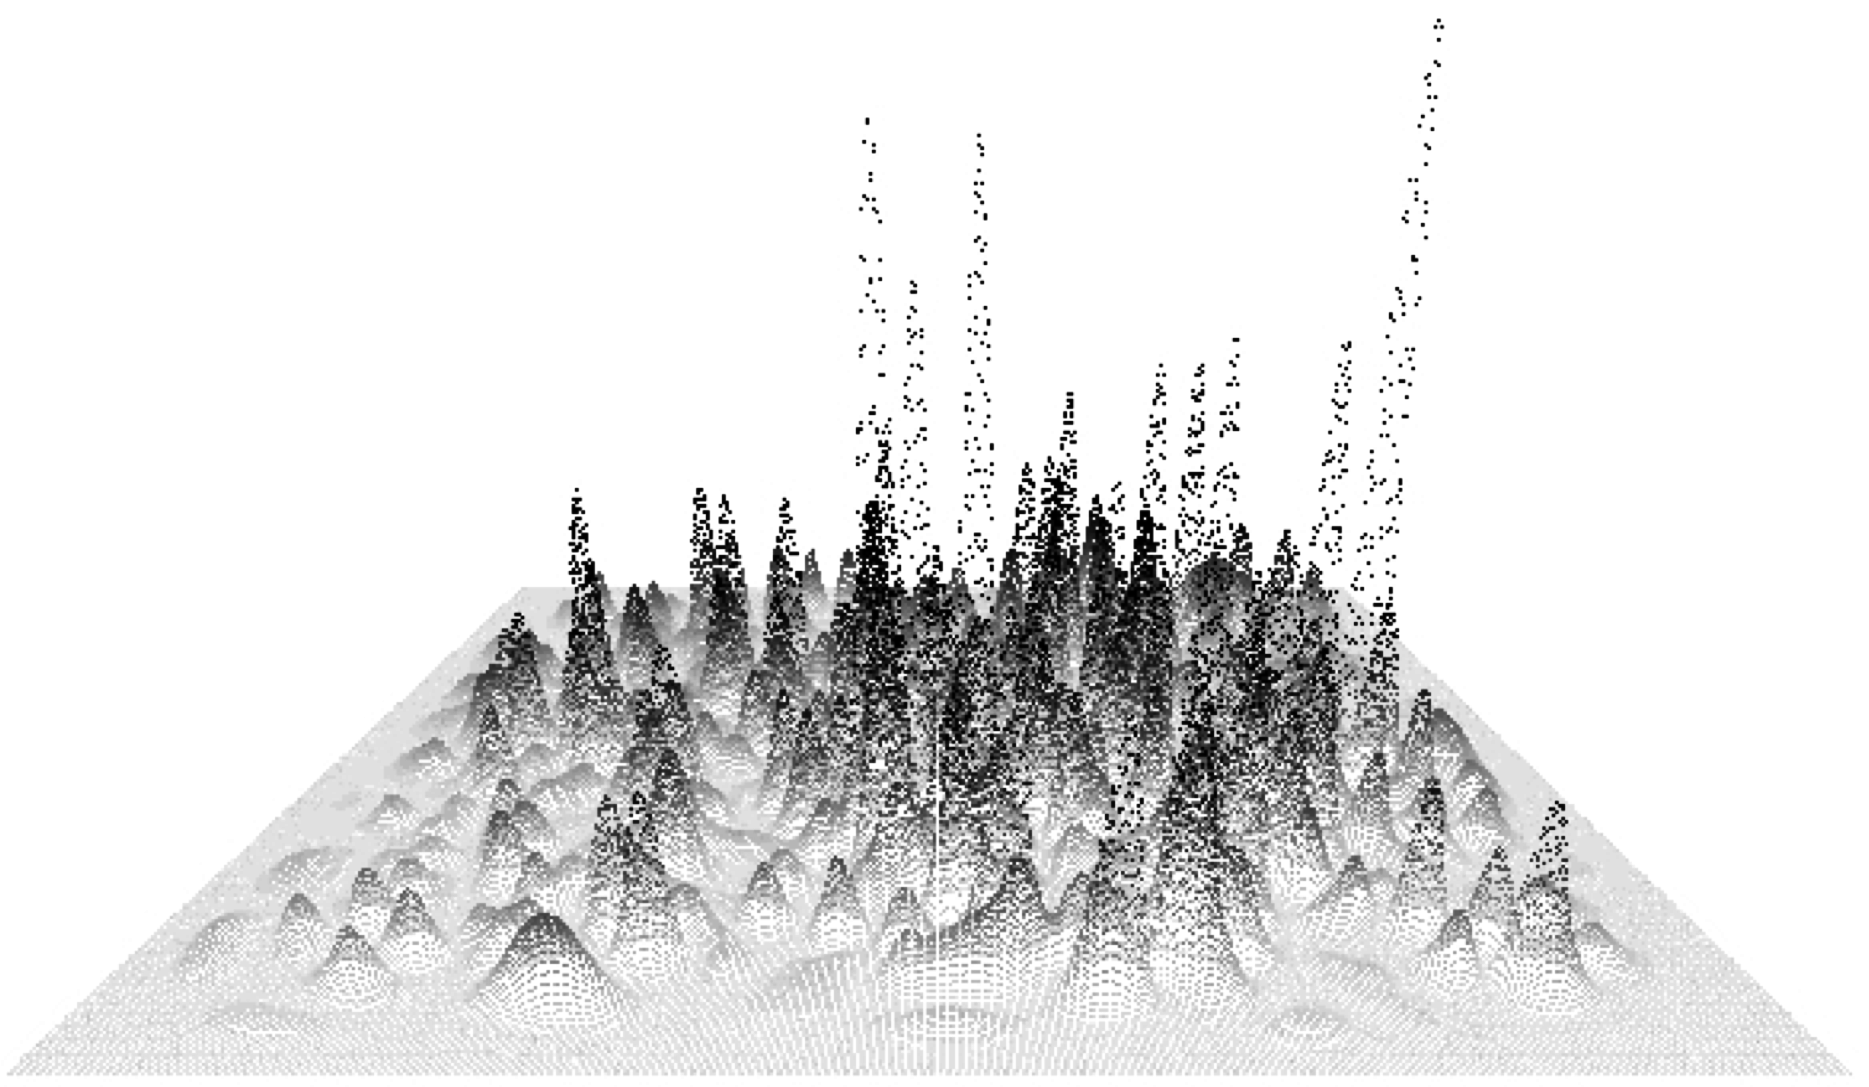
\includegraphics[width=\textwidth]{PPL/rl3.png}
  	\caption{\small The image shows a 3D representation of the intensity for the 2D electric field as computed by the SkelCL FDTD implementation after $60\,000$ iterations.}
	  \label{fig:fields}
  \end{minipage}
  \hspace{.02\textwidth}
  \begin{minipage}[b]{.48\textwidth}
    \centering
	  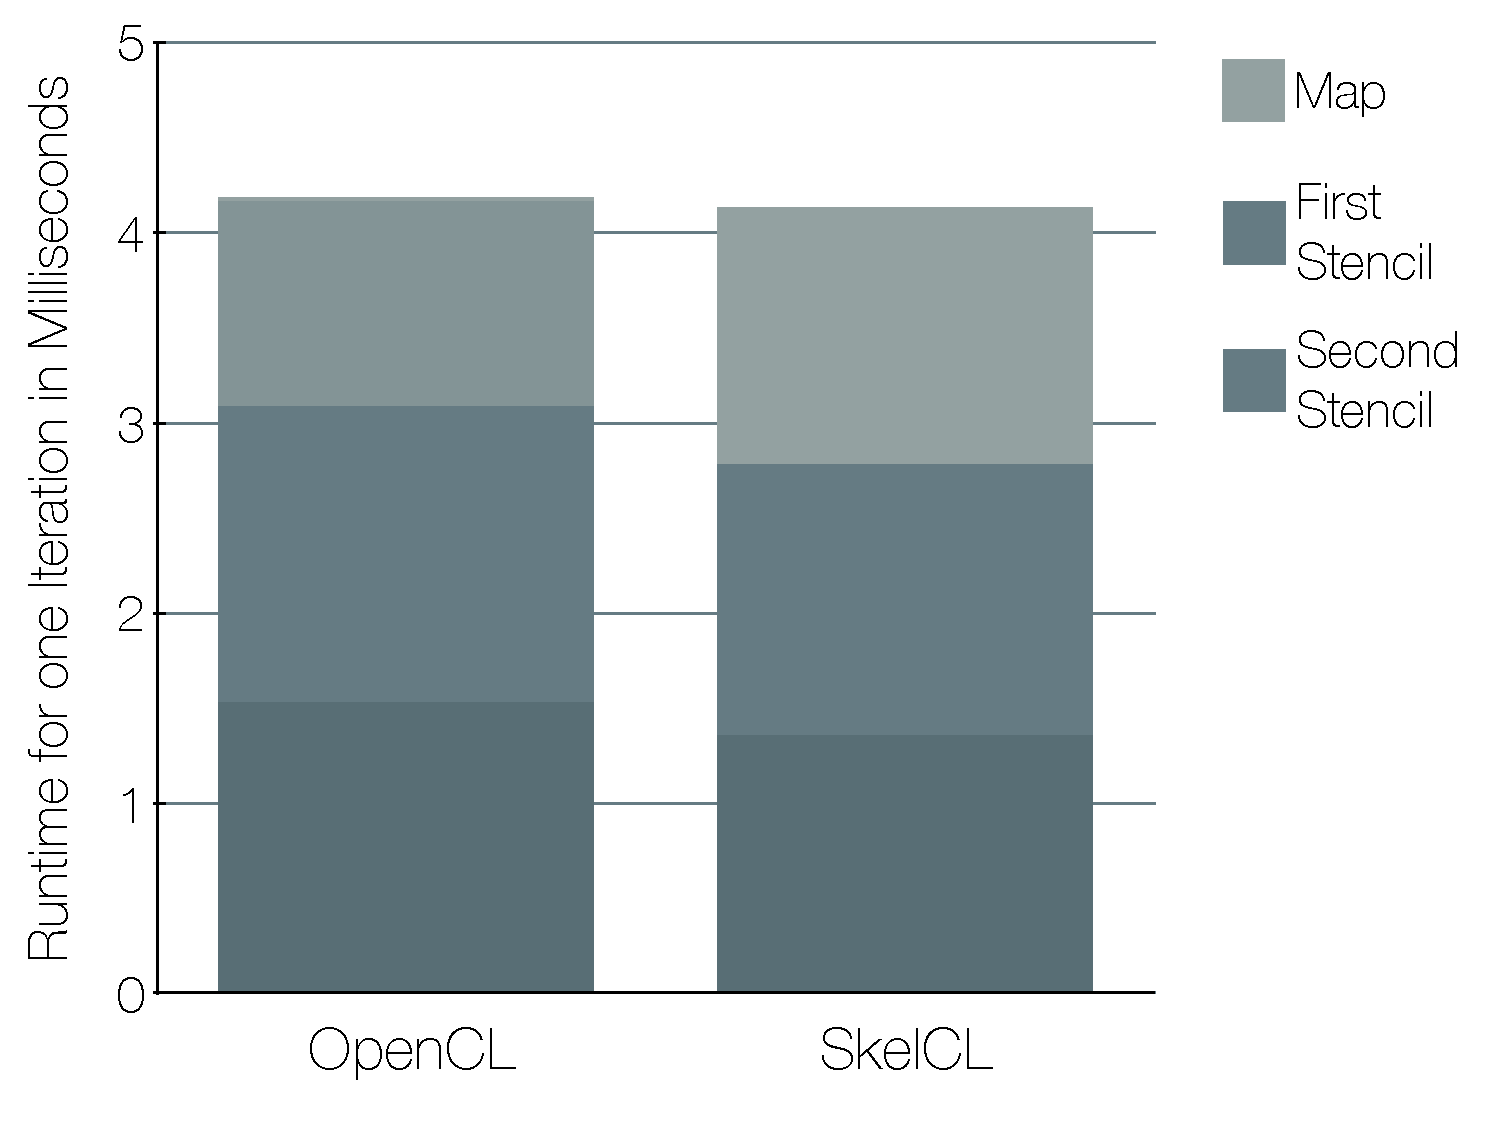
\includegraphics[width=\textwidth]{PPL/fdtd.pdf}
  	\caption{\small Runtime for one iteration of the FDTD application.}
  	\label{fig:fdtd_eval}
  \end{minipage}
  \bigskip
\end{figure}

\begin{figure}[tbp]
\begin{lstlisting}[%
  caption={Source code of the FDTD application in SkelCL},%
  label={lst:fdtd}]
Map<float4(float4)>     updateEnergyDist(...);
Stencil<float4(float4)> updateEField(...);
Stencil<float4(float4)> updateHField(
  "float4 func(float4_matrix_t E, float4_matrix_t H) { ... }");

Matrix<float4> N; // energy distribution in the medium
Matrix<float4> E; // E (electric) field
Matrix<float4> H; // H (magnetic) field

for (...) { // for each iteration
  updateEnergyDist(out(N), N, out(E));  
  updateEField(out(E), H, E);
  updateHField(out(H), E, H); }
\end{lstlisting}
\end{figure}

We implemented a two-dimensional version using SkelCL as well as a manually tuned OpenCL implementation.
To solve the PDEs (\ref{eq:rot_h}) and (\ref{eq:rot_d}), two separated three-point stencil computations are performed and one map computation for the gain-model is necessary.
Eq. (\ref{eq:div_e}) and (\ref{eq:div_h}) are implicitly solved by the FDTD method~\cite{Yee1966}.
Listing~\ref{lst:fdtd} shows the SkelCL code of the application:
in every iteration first the energy distribution is updated (line 11) using a map skeleton (defined in line 1);
then the first stencil (defined in line 2) updates the electric field $\vec{E}$ by combining a single element of $\vec{E}$ with three elements of the magnetic field $\vec{H}$ (line 12);
and finally the second stencil (defined in line 3) updates $\vec{H}$ by combining a single element of $\vec{H}$ with three elements of $\vec{E}$ (line 13).

Please note that the two stencil computations require both fields ($\vec{E}$ and $\vec{H}$) as input.
To implement this, we use the \emph{additional argument} feature of SkelCL which allows the additional field to be passed to skeletons on execution (see line 12 and 13).
The additional arguments are passed unchanged to the customizing function of the skeleton, therefore, the function customizing the stencil in line 4 now accepts $\vec{H}$ as a second parameter.
This feature greatly increases the flexibility of applications written in SkelCL.

In the evaluation we used a $2048 \times 2048$ sized matrix with a spatial resolution of $100$ cells per $\mu m$. 
This matrix corresponds to a square-shaped medium with the edge length of $20.1\,\mu m$. 
The medium size is actually smaller than the matrix size because of the border handling. 
To provide a physically correct simulation, the borders of the magnet field must be treated specially.
The Stencil skeleton provides sufficient functionality to allow for such border handling in the computation code.


We compared our SkelCL based implementation to a handwritten, fine-tuned OpenCL implementation which is based on \cite{Knitter2013}.
The OpenCL version is specifically designed for modern Nvidia GPUs.
In particular, it exploits the L1 and L2 caches of the Nvidia Fermi and Kepler architecture and does not explicitly make use of the local memory.
We performed the experiments on a system with a modern Nvidia K20c Kepler GPU with 5GB memory and 2496 compute cores.
Figure \ref{fig:fdtd_eval} shows the median times of a simulation time of $1\,ps$ equal to 60\, 000 iterations.
The SkelCL version slightly outperforms the OpenCL version by $2\%$.
The two stencil skeletons achieve ${\sim}10\%$ faster runtimes than the corresponding OpenCL kernels but the map skeleton is ${\sim}20\%$ slower, because it reads and writes all elements exactly once, while the customized OpenCL kernel does not write back all elements.
For this application it seems beneficial to make direct usage of the local memory as our implementation of the Stencil skeleton does, instead of relying on the caches of the hardware, as the OpenCL implementation does.

% This application study shows that real-world applications written in SkelCL can achieve the performance competitive with manually written OpenCL code.


\section{Bio Informatics}
\todo{Include gpuCup application}

\section{Conclusions}
\todo{Conclude}

